\chapter{Path Processing}%
\label{chap:path_processing}

	The sampling algorithm (Algorithm~\ref{alg:sampling_planning_overview})
	exits when it manages to attach the goal pose to the graph
	$\topologicalgraph$. At this point, a Dijkstra-search is performed on
	$\topologicalgraph$ to find an ordered set $\setofposes$ of poses $\pose$
	using the distance function in
	Equation~\ref{eq:distance_measure_capcity_margin} as the cost-to-go
	criterion.

	After this step, a collision-free path $\pathsym$ from the start to the goal
	pose may be found by taking points along the convex hull of subsequent
	points in the set $\setofposes$. The issue now becomes that the convex hull
	between two points is a straight line, which means that different segments
	of $\pathsym$ do not blend smoothly. Furthermore, due to the random nature
	of the sampling algorithm, the set $\setofposes$ may contain superfluous
	poses that will cause $\pathsym$ to be unnecessarily complicated. For this
	reason, several post-processing steps were developed and are discussed in
	the current chapter.

	\section{Path Simplification}%
\label{sec:path_simplification}

	A schematic example of the effect on $\pathsym$ of superfluous poses in
	$\setofposes$ can be seen in the left-hand side of
	Figure~\ref{fig:superfluous_poses}. The algorithms discussed here
	transform such a path into something more closely related to the
	right-hand side of the figure.

	Algorithms were developed to:

	\begin{enumerate}

		\item

			Remove unnecessary poses.

		\item

			Remove corners from the path.

		\item

			Reduce the total amount of rotation along the path.

	\end{enumerate}

	\begin{figure}[hb]
		\centering
		\def\svgwidth{\columnwidth}
		\import{res/img/}{superfluous_poses.pdf_tex}
		\caption{Superfluous Pose Removal}%
		\label{fig:superfluous_poses}
	\end{figure}

	\subsection{Pose Removal}%
	\label{sec:pose_removal}

		A simple recursive algorithm was developed to remove poses from
		$\setofposes$. The pseudocode is given in
		Algorithm~\ref{alg:pose_removal}.

		\begin{algorithm}[ht]
			\caption{Pose Removal}
			\label{alg:pose_removal}
			\begin{algorithmic}[1]
				\Procedure{Remove\_Poses}{}
					\State{}\code{simplified = false}
					\For{$\indexi \in [0, |\setofposes| -2]$}
						\If{$\dist(\pose_{\indexi}, \pose_{\indexi+2}) >
						\dist(\pose_{\indexi}, \pose_{\indexi+1})$}%
						\label{alg:pose_removal:distance_check}
							\If{$\code{Farthest\_Collision\_Free\_Point}(\pose_{\indexi},
							\pose_{\indexi+2}) = \pose_{\indexi+2}$}
								\State{}Remove $\pose_{\indexi+1}$ from
								$\setofposes$
								\State{}$\code{simplifed = true}$
							\EndIf{}
						\EndIf{}
					\EndFor{}
					\If{\code{simplified}}
						\State{}\code{Remove\_Poses}
					\EndIf{}
				\EndProcedure{}
			\end{algorithmic}
		\end{algorithm}

		This algorithm simply removes an intermediate pose if the pose
		before and after it in the sequence in $\setofposes$ can be
		connected by a straight line. However, since a Euclidean distance
		measure (Equation~\ref{eq:euclidean_distance}) is not used, a path
		may actually be \textit{shorter} if an additional intermediate point
		is inserted between two points. For this reason, the algorithm only
		removes points if this would reduce the total travelled distance
		of the path. This is achieved by using the distance measure
		(Equation~\ref{eq:distance_measure_capcity_margin}) in
		Line~\ref{alg:pose_removal:distance_check}.

	\subsection{Corner Removal}%
	\label{sec:corner_removal}

		In some instances, a path cannot be shortened by removing a pose
		from $\setofposes$, since the resulting path would be in collision.
		In such cases, the path may often contain a corner that may be far
		away from the rest of the path. Figure~\ref{fig:path_corner} shows
		a schematic example of this case. To deal with this, an algorithm
		was developed to remove such corners.

		\begin{figure}[hb]
			\centering
			\def\svgwidth{\columnwidth}
			\import{res/img/}{corner_removal.pdf_tex}
			\caption{Path Corner}
			\label{fig:path_corner}
		\end{figure}

		The algorithm tries to find the points $\pose_a, \pose_b$ that
		minimises the total distance travelled along the segment:

		\begin{equation}
			(\pose_a, \pose_b) = \argmin
				(
					\dist(\pose_1, \pose_a) +
					\dist(\pose_a, \pose_b) +
					\dist(\pose_b, \pose_3)
				)
		\end{equation}

		Subject to the constraint:

		\begin{equation}
			\forall
				\obstacle
			\forall
			(
				\pose\in
				\convexhull(\pose_1, \pose_a) \cup \convexhull(\pose_a,
				\pose_b) \cup \convexhull(\pose_b, \pose_3)
			)
			\quad\robot(\pose) \cap \obstacle = \emptyset
		\end{equation}

		This is done by writing the convex hull between two poses as a
		parametric line:

		\begin{align}
			\linevec_1 &= \pose_1 + \timenorm_a(\pose_2 - \pose_1)\\
			\linevec_2 &= \pose_3 + \timenorm_b(\pose_2 - \pose_3)\\
		\end{align}

		Now, using a simple linear search on both $\timenorm_a$ and
		$\timenorm_b$, find the minimum values, $\timenorm_a',
		\timenorm_b'$, for which:

		\begin{align}
			\robot(\convexhull(\pose_1, \linevec_2(\timenorm_b))) \cap
				\obstacle = \emptyset\\
			\robot(\convexhull(\pose_3, \linevec_1(\timenorm_a))) \cap
				\obstacle = \emptyset
		\end{align}

		Now, a two-dimensional binary search is performed on $\timenorm_a$
		and $\timenorm_b$ in the ranges:

		\begin{align}
			\timenorm_a \in [\timenorm_a', 1]\\
			\timenorm_b \in [\timenorm_b', 1]
		\end{align}

		Which produce the poses $\pose_a$ and $\pose_b$ which minimises the
		distance expression and satisfies the constraints of the problem.

	\subsection{Rotation Optimisation}%
	\label{sec:rotation_optimisation}

		Due to the rotation sampling strategy employed as discussed in
		Section~\ref{sec:sample_strategy}, the orientations of the end-effector
		throughout its trajectory will be upright and tend to avoid
		unnecessarily large rotations. However, there may still be some residual
		oscillations around the $y$ axis during its motion. For this reason,
		it is worthwhile to employ a rotation optimisation step.

		The rotation optimisation algorithm uses quaternion
		\gls{slerp}~\cite{bib:math:a_compact_differential_formula_for_the_first_derivative_of_a_unit_quaternion_curve}%
		\cite{bib:math:a_general_construction_scheme_for_unit_quaternion_curves_with_simple_high_order_derivatives}.
		It is summarised in Algorithm~\ref{alg:rotation_optimisation}.

		\begin{algorithm}[ht]
			\caption{Rotation Optimisation}
			\label{alg:rotation_optimisation}
			\begin{algorithmic}[1]
				\Procedure{Optimise\_Rotations}{}
					\ForAll{$%
						\pose_{\indexi} \in
							\setofposes\setminus
								(\pose_{\initial}, \pose_{\goal})
					$}
						\State{}%
							$
								\pose_{\indexi}' \gets
									\code{slerp\_interpolate}
									(
										0.5,
										\pose_{\indexi - 1},
										\pose_{\indexi},
										\pose_{\indexi + 1}
									)
							$
							\label{alg:rotation_optimisation:slerp}
						\If{$
							\dist(\pose_{\indexi - 1}, \pose_{\indexi}') +
							\dist(\pose_{\indexi}', \pose_{\indexi + 1})
							\leq
							\dist(\pose_{\indexi - 1}, \pose_{\indexi}) +
							\dist(\pose_{\indexi}, \pose_{\indexi + 1})
						$}
							\If{$
								\code{path\_okay}
									(
										\pose_{\indexi - 1},
										\pose_{\indexi}',
										\pose_{\indexi + 1}
									)
							$}
								\State{}%
									$
										\pose_{\indexi} \gets \pose_{\indexi}'
									$
							\EndIf{}
						\EndIf{}
					\EndFor{}
				\EndProcedure{}
			\end{algorithmic}
		\end{algorithm}

		The algorithm simply iterates over all the poses in the set and attempts
		to adjust the rotation of each pose so that it is between the rotations
		of the poses that precede and follow it. This is done by
		Line~\ref{alg:rotation_optimisation:slerp}, which returns a pose
		$\pose_{\indexi}'$ that has the same translation component as
		$\pose_{\indexi}$, but whose quaternion is the midway point of the
		\gls{slerp} of poses $\pose_{\indexi - 1}$ and $\pose_{\indexi + 1}$.

		The rotation optimisation algorithm could be run multiple times on
		$\setofposes$ to obtain a progressively more linear rotation progression
		from $\pose_{\initial}$ to $\pose_{\goal}$. However, due to the other
		simplification algorithms, the number of poses in $\setofposes$ tends to
		be small and repeated execution is usually not necessary. Furthermore,
		due to the necessity to check collisions, repeatedly running
		Algorithm~\ref{alg:rotation_optimisation} does get expensive quickly.

	\subsection{Increasing the Capacity Margin}%
	\label{sec:increasing_the_capacity_margin}

		At this point a set $\setofposes$ has been found that is guaranteed to
		be collision-free. However, due to the random nature of the path search
		algorithm, little is done to optimise the overall capacity margin
		$\capacitymargin$ of the trajectory. Two approaches to improve the
		capacity margin are proposed:

		\begin{enumerate}

			\item
				Change the condition for the collision detection algorithm.
				\label{option:change_collision_condition}

			\item
				Post-process $\setofposes$ to improve $\capacitymargin$.
				\label{option:post_process_set_of_poses}

		\end{enumerate}

		Option~\ref{option:change_collision_condition} is to define some minimum
		threshold capacity margin ${\capacitymargin}_{\tol}$ and modify the
		capacity margin submodule ${\logicalpredicate}_{\capacitymargin}$ of the
		collision detection algorithm as follows:

		\begin{equation}
			{\logicalpredicate}_{\capacitymargin} =
				\begin{cases}
					\false, \quad \capacitymargin > {\capacitymargin}_{\tol} \\
					\true, \quad \text{otherwise}
				\end{cases}
		\end{equation}

		This will guarantee that at each point in the trajectory the capacity
		margin is above this minimum limit.

		Option~\ref{option:post_process_set_of_poses} requires that each pose be
		changed according to:

		\begin{equation}
			\forall
				\left(
					{\pose}_{\indexi} \neq {\pose}_{\initial}, {\pose}_{\goal}
				\right)
			\in
				\setofposes,
			%
			{\pose}_{\indexi}' \gets
				{\pose}_{\indexi} + {\gain}_{\indexi}\nabla\capacitymargin({\pose}_{\indexi})
			\label{eq:capacity_margin_increase}
		\end{equation}

		Here, the gain ${\gain}_{\indexi}$ determines how far to move
		${\pose}_{\indexi}$ in the direction of increasing $\capacitymargin$. Of
		course, this is subject to the constraints:

		\begin{equation}
			\dist_{\pathsym}
				\left(
					{\pose}_{\indexi - 1},
					{\pose}_{\indexi}'
				\right)
			+
			\dist_{\pathsym}
				\left(
					{\pose}_{\indexi}',
					{\pose}_{\indexi + 1}
				\right)
			<
			\dist_{\pathsym}
				\left(
					{\pose}_{\indexi - 1},
					{\pose}_{\indexi}
				\right)
			+
			\dist_{\pathsym}
				\left(
					{\pose}_{\indexi},
					{\pose}_{\indexi + 1}
				\right)
			\label{eq:constraint_shorter_distance}
		\end{equation}

		and

		\begin{equation}
			\logicalpredicate(\pathsym') = \false
			\label{eq:constraint_no_collision}
		\end{equation}

		These constraints essentially require that the distance found be shorter
		due to an increase in capacity margin, but still be free of collisions.

		Due to the costs involved in evaluating
		Constraint~\ref{eq:constraint_shorter_distance}, the search on
		${\gain}_{\indexi}$ should be limited. As such, it is beneficial to
		define a discrete set ${{\gain}_{\indexi}}_1 \ldots
		{{\gain}_{\indexi}}_n$ for which
		Equation~\ref{eq:capacity_margin_increase} is called.  If this set of
		gains is kept small, the procedure can be run multiple times to search
		for a path with a higher capacity margin. Of course, this has a
		trade-off with the overall calculation time required.

	\section{Smooth Interpolation}%
\label{sec:smooth_interpolation}

	After the path has been simplified using the algorithms described in
	Section~\ref{sec:path_simplification}, a path consisting of straight lines
	with hard corners is obtained. The next step is to generate a smoother
	trajectory that approximates the path while still avoiding obstacles.
	Figure~\ref{fig:path_smoothing} shows a schematic representation of the
	desired output.

	\begin{figure}[hb]
		\centering
		\def\svgwidth{\columnwidth}
		\import{res/img/}{smoothed_path.pdf_tex}
		\caption{Path Smoothing}%
		\label{fig:path_smoothing}
	\end{figure}

	B-spline curves were used to obtain the desired trajectory. To achieve this,
	each pose $\pose$ in the ordered set of poses $\setofposes$ in the
	simplified path is considered as a control point of the final B-spline
	trajectory. The trajectory is then generated using the well-known B-spline
	recursive relation repeated here for
	completeness~\cite{bib:math:spline_notes}:

	\begin{align}
		\begin{split}
			\pathsym(\timesym) &=
				\sum^{|\setofposes|}_{i=0} N_{i, k}(\timesym)\pose_{\indexi}\\
			%%%%
			N_{\indexi, \indexj}(\timesym) &=
				\frac
				{%
					\timesym - \timesym_{\indexi}
				}
				{%
					\timesym_{\indexi + \indexj} - \timesym_{\indexi}
				}
				N_{\indexi, \indexj - 1}
				+
				\frac
				{%
					\timesym_{\indexi + \indexj + 1} - \timesym
				}
				{%
					\timesym_{\indexi + \indexj + 1} - \timesym_{\indexi + 1}
				}
				N_{\indexi + 1, \indexj - 1}\\
			%%%%%
			N_{\indexi, 0}(\timesym) &=
				\begin{cases}
					1, \quad \timesym_{\indexi} \leq \timesym < \timesym_{\indexi + 1}\\
					0, \quad \text{otherwise}
				\end{cases}\\
			%%%%%
			\vec{\timesym} &=
				\left[
					\begin{matrix}
						\timesym_0, \ldots, \timesym_{k + |\setofposes| + 1}
					\end{matrix}
				\right]
		\end{split}
		\label{eq:b_spline_recursion}
	\end{align}

	Where $k$ is the degree of the B-spline used to approximate the points in
	$\setofposes$ and $\vec{\timesym}$ is the equidistant knot vector that
	produces the uniform spline.

	\subsection{Guaranteeing Smooth Path Safety}%
	\label{sec:guaranteeing_smooth_path_safety}

		Blindly applying Equation~\ref{eq:b_spline_recursion} makes no guarantee
		that the smooth path will be collision free. The generated spline curve
		must therefore be checked for collisions and corrective action must be
		taken in the case that a new collision is detected.

		One technique that is commonly used with B-spline curves is that of knot
		multiplicity. The elements in the knot vector $\vec{\timesym}$ are
		generally spaced equidistantly~\cite{bib:math:spline_notes}. However,
		the multiplicity of a knot may be increased by letting consecutive knots
		assume the same value. This has the effect of drawing the spline closer
		to a control point, but also drops a degree of differentiability at this
		point. A schematic representation of this effect can be seen in
		Figure~\ref{fig:knot_multiplicity}.

		\begin{figure}[hb]
			\centering
			\def\svgwidth{\columnwidth}
			\import{res/img/}{knot_multiplicity.pdf_tex}
			\caption{Increased Knot Multiplicity}%
			\label{fig:knot_multiplicity}
		\end{figure}

		While such an approach works, it presents some drawbacks:

		\begin{itemize}

			\item Loss of smoothness.

				A goal of this thesis is to generate smooth trajectories.
				Dropping a degree of differentiability can create
				discontinuities in the jerk, acceleration or velocity profiles
				of the final trajectory. In the worst case, if a point in the
				path degenerates to $\contdeggeom{0}$ --- that is, a hard corner
				in the position profile --- the end-effector would have to come
				to a complete stop at this point and then accelerate from rest
				again. Stopping the motion in the middle of the trajectory is a
				non-ideal approach and should be avoided as much as possible.

			\item Slow Computation Time.

				In general, higher-degree B-spline curves may be used to
				generate a path in configuration space. If part of the curve is
				in collision, then the multiplicity of the point must be
				increased and the path must be checked again. The path can
				potentially still be in collision and, consequently, this
				process can repeat until the offending point degenerates to
				$\contdeggeom{0}$.

		\end{itemize}

		Instead, this thesis proposes to augment $\setofposes$ with additional
		poses such that the spline curve generated from
		Equation~\ref{eq:b_spline_recursion} is guaranteed to be free of
		collisions. This is achieved by noticing from
		Equation~\ref{eq:b_spline_recursion} that any point in $\pathsym$ is
		obtained from convex combinations of subsequent poses. This means that
		the path is guaranteed to go through the convex hull of the currently
		active control points. The consequence of this is that, if the hull of
		the points can be shown to be collision-free, then the path is
		guaranteed to be collision free automatically. The algorithm developed
		is reported in Algorithm~\ref{alg:set_of_poses_augmentation}.

		\begin{algorithm}[ht]
			\caption{$\setofposes$ Augmentation}%
			\label{alg:set_of_poses_augmentation}
			\begin{algorithmic}[1]
				\Procedure{Augment\_Pose\_Set}{\setofposes{}}
					\State{}Declare new set $\setofposes'$
					\State{}Add first pose in $\setofposes$ to $\setofposes'$
					\ForAll{$\pose_{\indexi} \in \setofposes\setminus
					\pose_{\initial}, \pose_{\goal}$}
						\State{}$\pose_0 = \pose_{\indexi - 1}$
						\State{}$\pose_1 = \pose_{\indexi}$
						\State{}$\pose_2 = \pose_{\indexi + 1}$
						\State{}$\timenorm_1 = 0$
						\State{}$\timenorm_2 = 1$
						\While{$\timenorm_1 \leq 0.5$ and $\timenorm_2 \geq 0.5$}
							\State{}$\pose_a = \pose_0 + \timenorm_1(\pose_1 -
								\pose_0)$
							\State{}$\pose_b = \pose_1 + \timenorm_2(\pose_2 -
								\pose_1)$
							\State{}$\timenorm_1 = \timenorm_1 + \Delta\timenorm$
							\State{}$\timenorm_2 = \timenorm_2 - \Delta\timenorm$
							\If{Farthest\_Collision\_Free\_Point($\pose_a, \pose_b)= \pose_b$}
								\State{}break
							\EndIf{}
						\EndWhile
						\State{}$\setofposes'\code{.push}(\pose_a, \pose_1, \pose_b)$
					\EndFor{}
					\State{}Add last point in $\setofposes$ to $\setofposes'$
					\State{}return $\setofposes'$
				\EndProcedure
			\end{algorithmic}
		\end{algorithm}

		A graphical intuition of Algorithm~\ref{alg:set_of_poses_augmentation}
		can be seen in Figure~\ref{fig:set_of_poses_augmentation}. Essentially,
		it tries to find a shorter straight-line path
		$\vecline{\pose_a}{\pose_b}$ that connects poses $\pose_0$ and
		$\pose_2$, but cuts out $\pose_1$. The search is performed by moving
		$\pose_a$ from $\pose_0$ to the midpoint of the line
		$\vecline{\pose_0}{\pose_1}$ and $\pose_b$ from the midpoint of
		$\vecline{\pose_1}{\pose_2}$ to $\pose_1$.

		\begin{figure}[hbt]
			\centering
			\def\svgwidth{0.7\columnwidth}
			\import{res/img/}{subdivide_control_points.pdf_tex}
			\caption{$\setofposes$ Augmentation}%
			\label{fig:set_of_poses_augmentation}
		\end{figure}

		A shorter path could potentially be found by varying $\timenorm_1$ and
		$\timenorm_2$ in nested loops. However, the call to
		\code{Farthest\_Collision\_Free\_Point} is quite expensive. Nested loops
		would mean that the function is called
		\(
			O
			\left(
				\ceil*
				{%
					{%
						\left(
							\frac
							{%
								1
							}
							{%
								2\Delta\timenorm
							}
						\right)
					}^2
				}
			\right)
		\)
		times, instead of just
		\(
			O
			\left(
				\ceil*
				{%
					\left(
						\frac
						{%
							1
						}
						{%
							2\Delta\timenorm
						}
					\right)
				}
			\right)
		\)
		times. Note here that we require $\Delta\timenorm \in (0, 1]$.
		Therefore, the algorithm in its presented state represents a tradeoff
		between speed and path-length.

		A B-spline curve created using Equation~\ref{eq:b_spline_recursion} on
		the augmented set $\setofposes'$ generated from
		Algorithm~\ref{alg:set_of_poses_augmentation} can be viewed as a set of
		straight lines smoothly interpolated with polynomial bends. The
		algorithm has the following benefits:

		\begin{itemize}

			\item Fast

				The algorithm is linear in the amount of times that the
				collision algorithm needs to be called.

			\item Smooth

				The algorithm ensures that sampled points are connected with the
				maximum degree of smoothness that can be achieved by the degree
				chosen for the B-spline curve.
		\end{itemize}

		A schematic representation of the effect of augmenting $\setofposes$ can
		be seen in Figure~\ref{fig:set_of_poses_augmentation_path}. Note that
		although the figure is schematic in nature, it is drawn using B-spline
		curves and control points as discussed in this section.  As can be seen
		in the figure, adding additional control poses $\pose_a$ and $\pose_b$,
		a collision with $\configurationspace_{\obstacleregion}$ can be avoided
		while still maintaining the smoothness of the curve.

		\begin{figure}[hb]
			\centering
			\def\svgwidth{\columnwidth}
			\import{res/img/}{augmented_control_points.pdf_tex}
			\caption{Effecto of $\setofposes$ Augmentation on $\pathsym$}
			\label{fig:set_of_poses_augmentation_path}
		\end{figure}

	\section{Sample Path Processing Output}%

	Figure~\ref{fig:sample_planning_problem} shows some screenshots of the
	trajectory generation software developed. In the figure, several views
	of a planning problem in a cluttered environment are shown. As can be
	seen, the problem contains obstacles on the ground, on the sides of the
	workspace, as well as hanging from the top of the workspace. The goal is
	to move the end-effector from the start position shown in the figures to
	the opposite corner of the workspace while avoiding collisions.

	\begin{figure}[hbt]
		\centering
		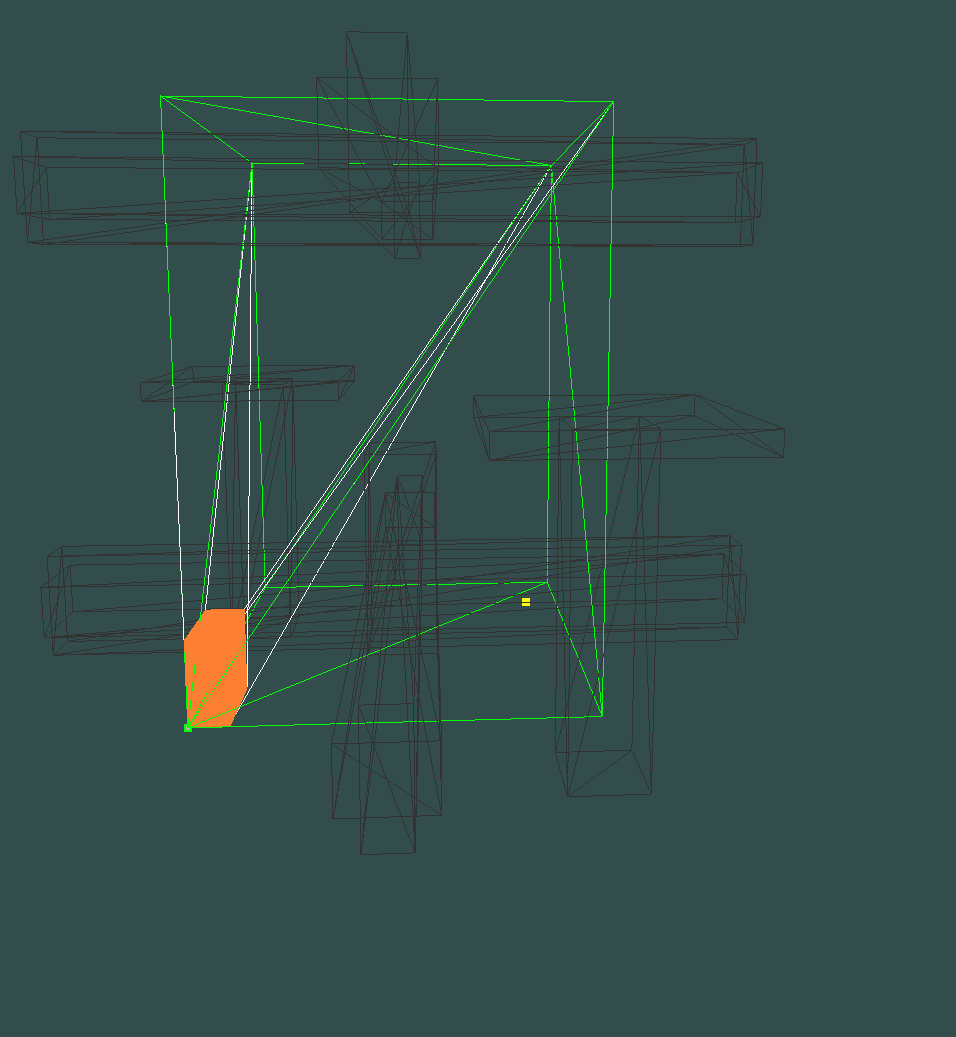
\includegraphics[width=0.3\linewidth]{clutter_front.png}
		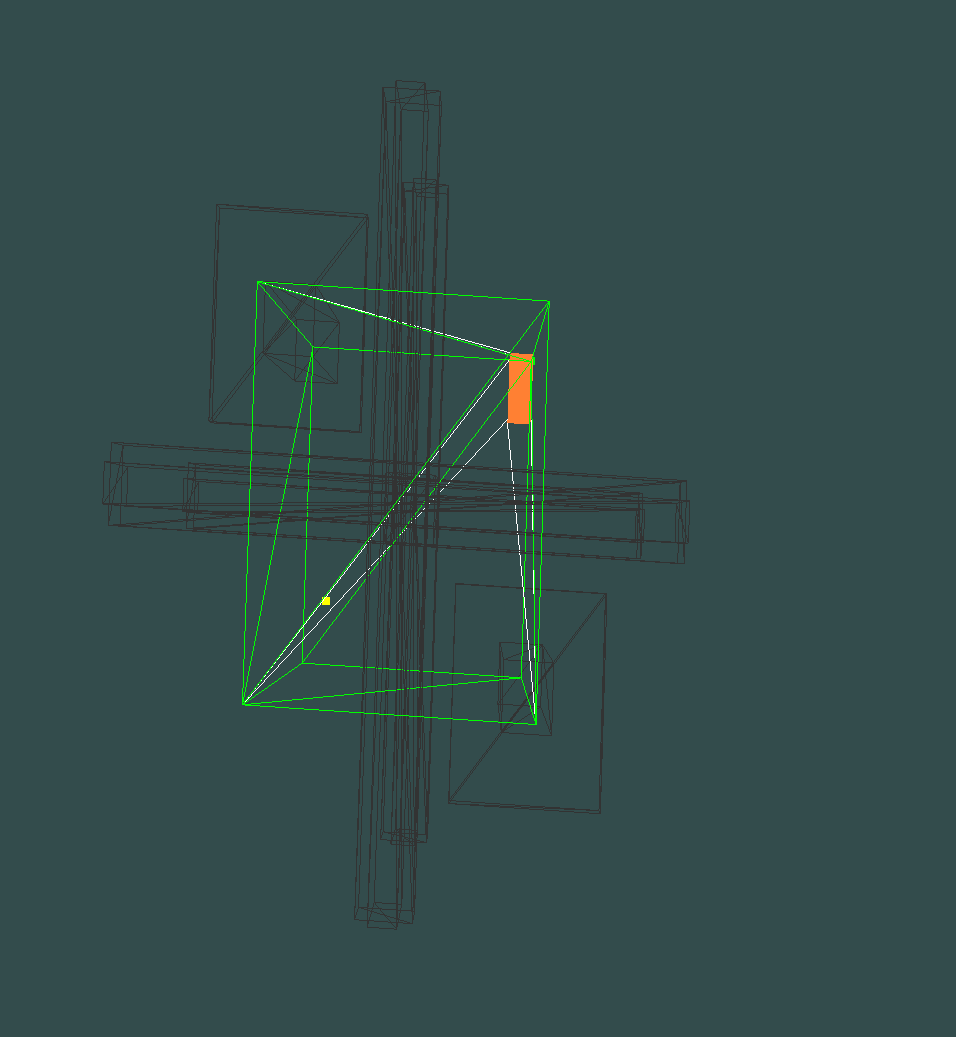
\includegraphics[width=0.3\linewidth]{clutter_top.png}
		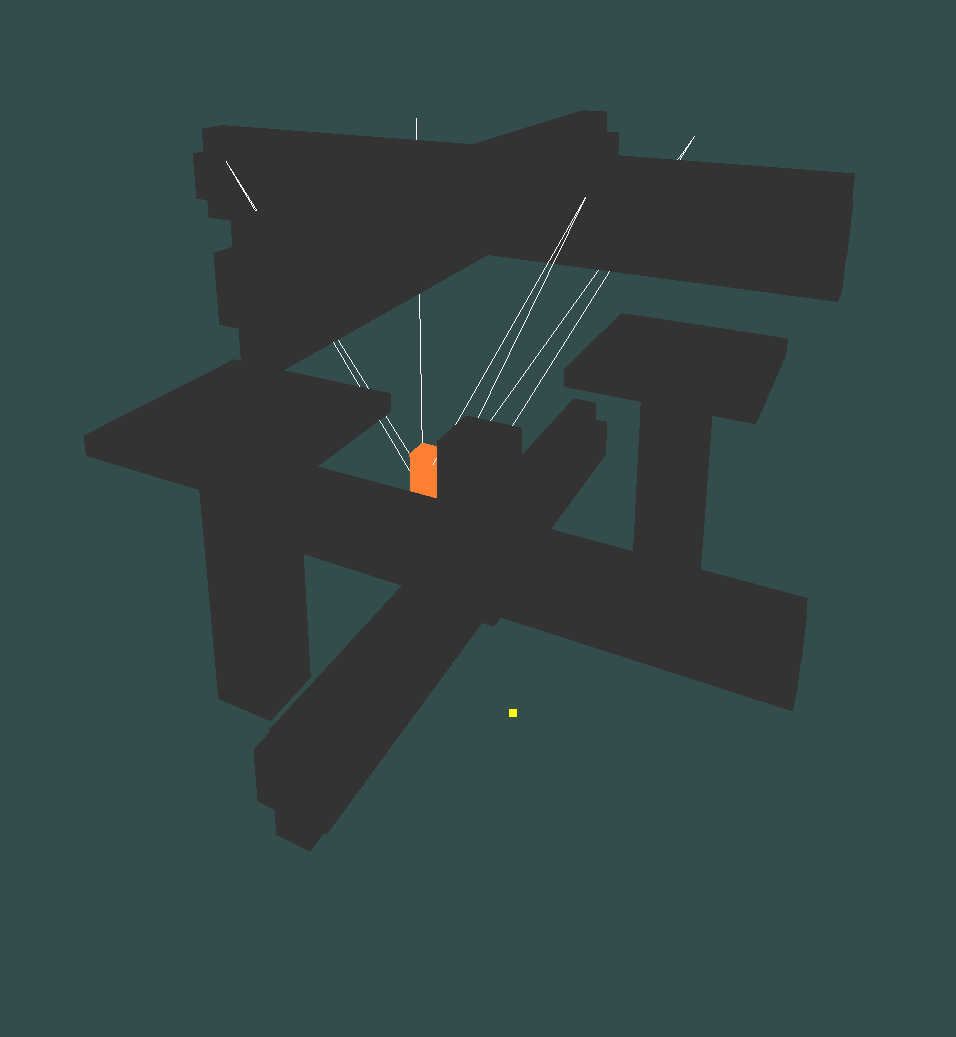
\includegraphics[width=0.3\linewidth]{clutter_perspective.png}
		\caption{Sample Planning Problem}
		\label{fig:sample_planning_problem}
	\end{figure}

	The software was asked to find a collision-free B-spline path of degree 8
	for the problem shown in Figure~\ref{fig:sample_planning_problem}. Different
	stages in the path-processing stage of the planning is reported in
	Figures~\ref{fig:sample_trajectory_after_simplification}
	and~\ref{fig:sample_trajectory_with_augmented_set_of_poses}.

	%\begin{figure}[hb]
	%	\centering
	%	\begin{minipage}{\linewidth}
	%		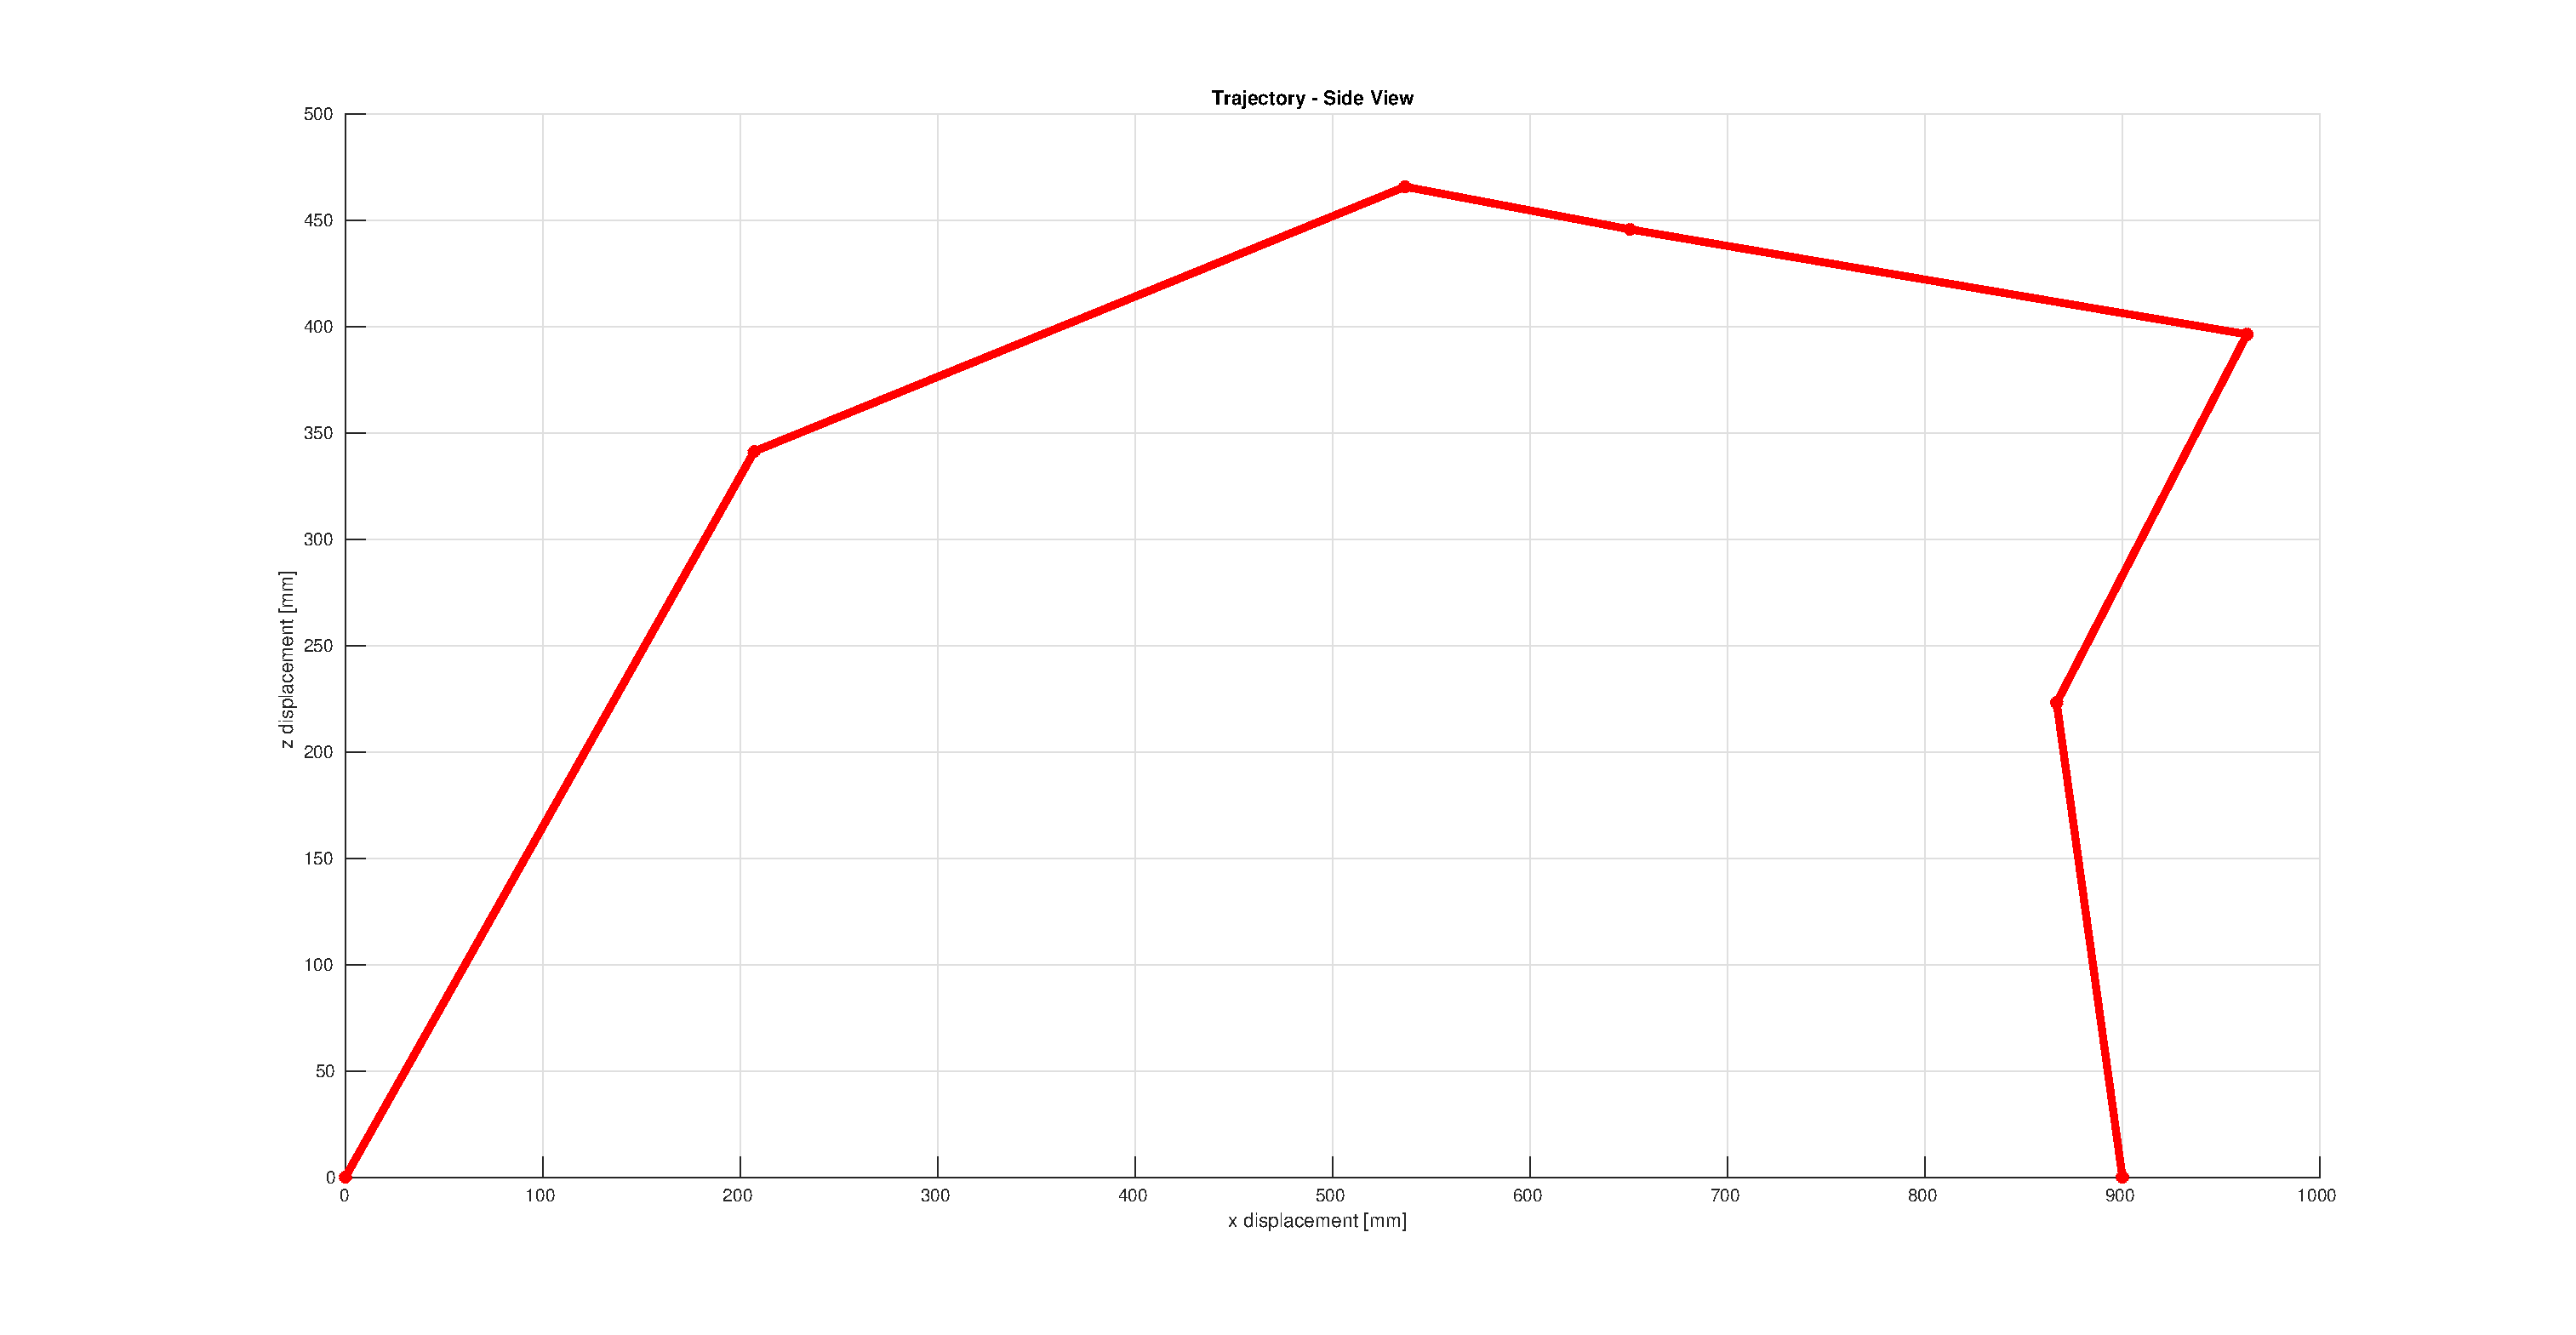
\includegraphics[height=0.45\linewidth, width=0.45\linewidth]{trajectory_no_simplify_side.eps}
	%		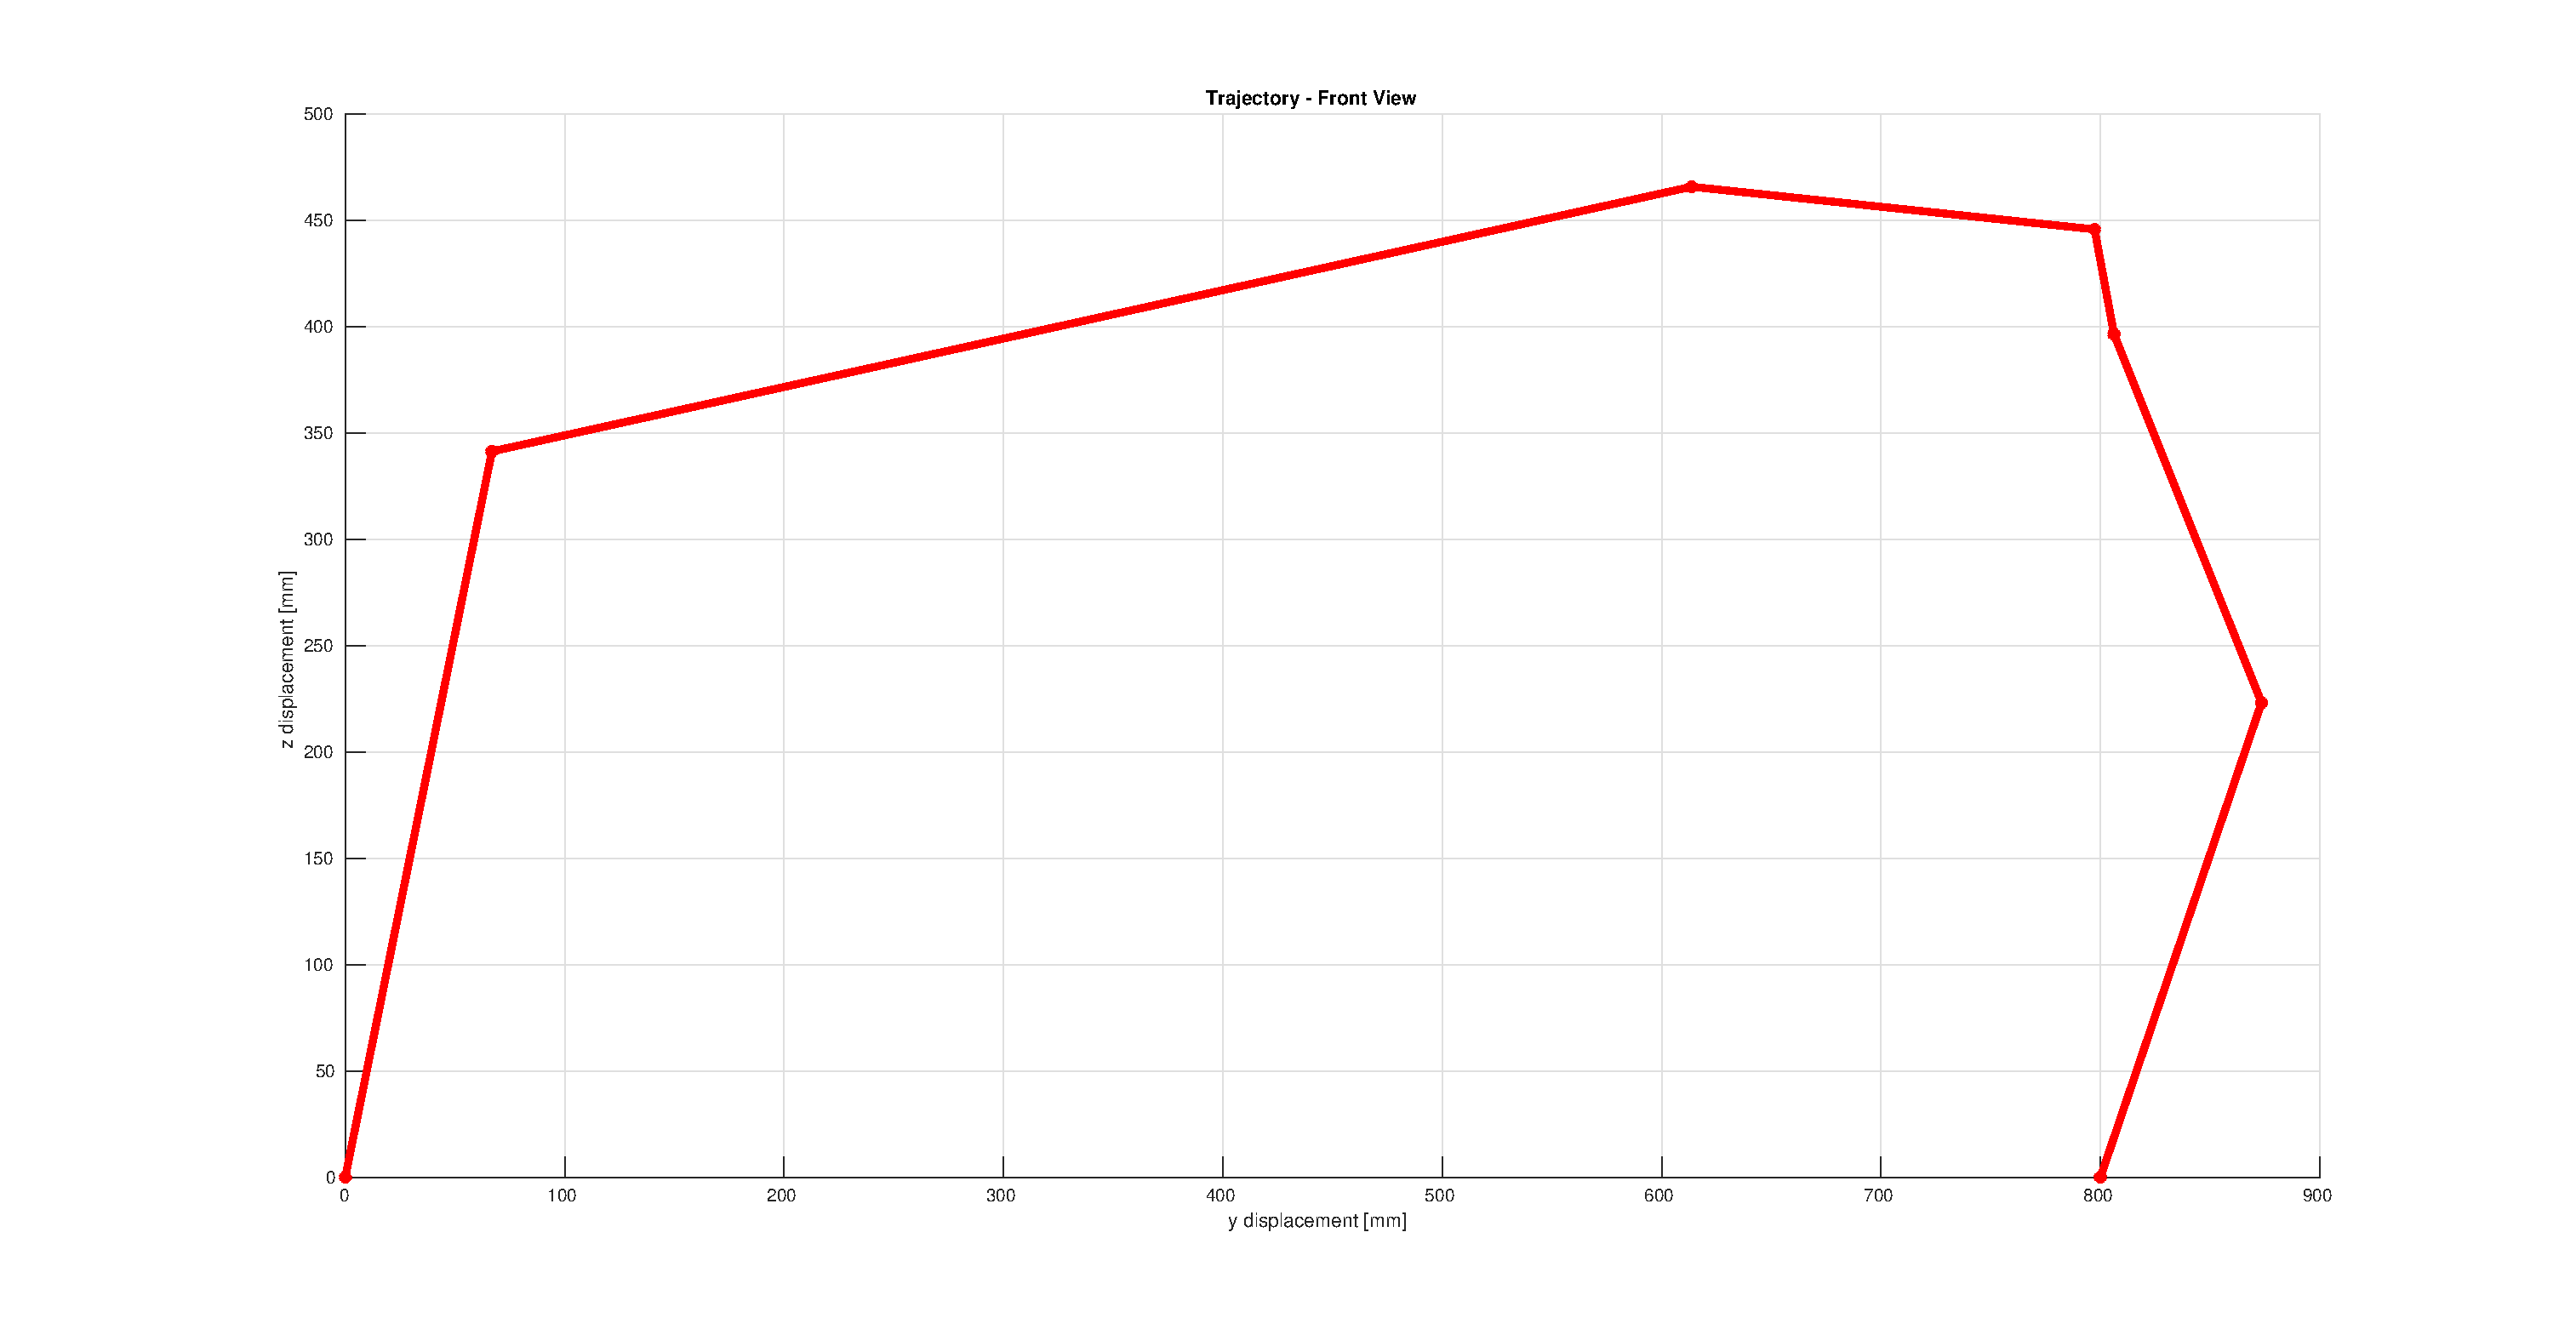
\includegraphics[height=0.45\linewidth, width=0.45\linewidth]{trajectory_no_simplify_front.eps}
	%		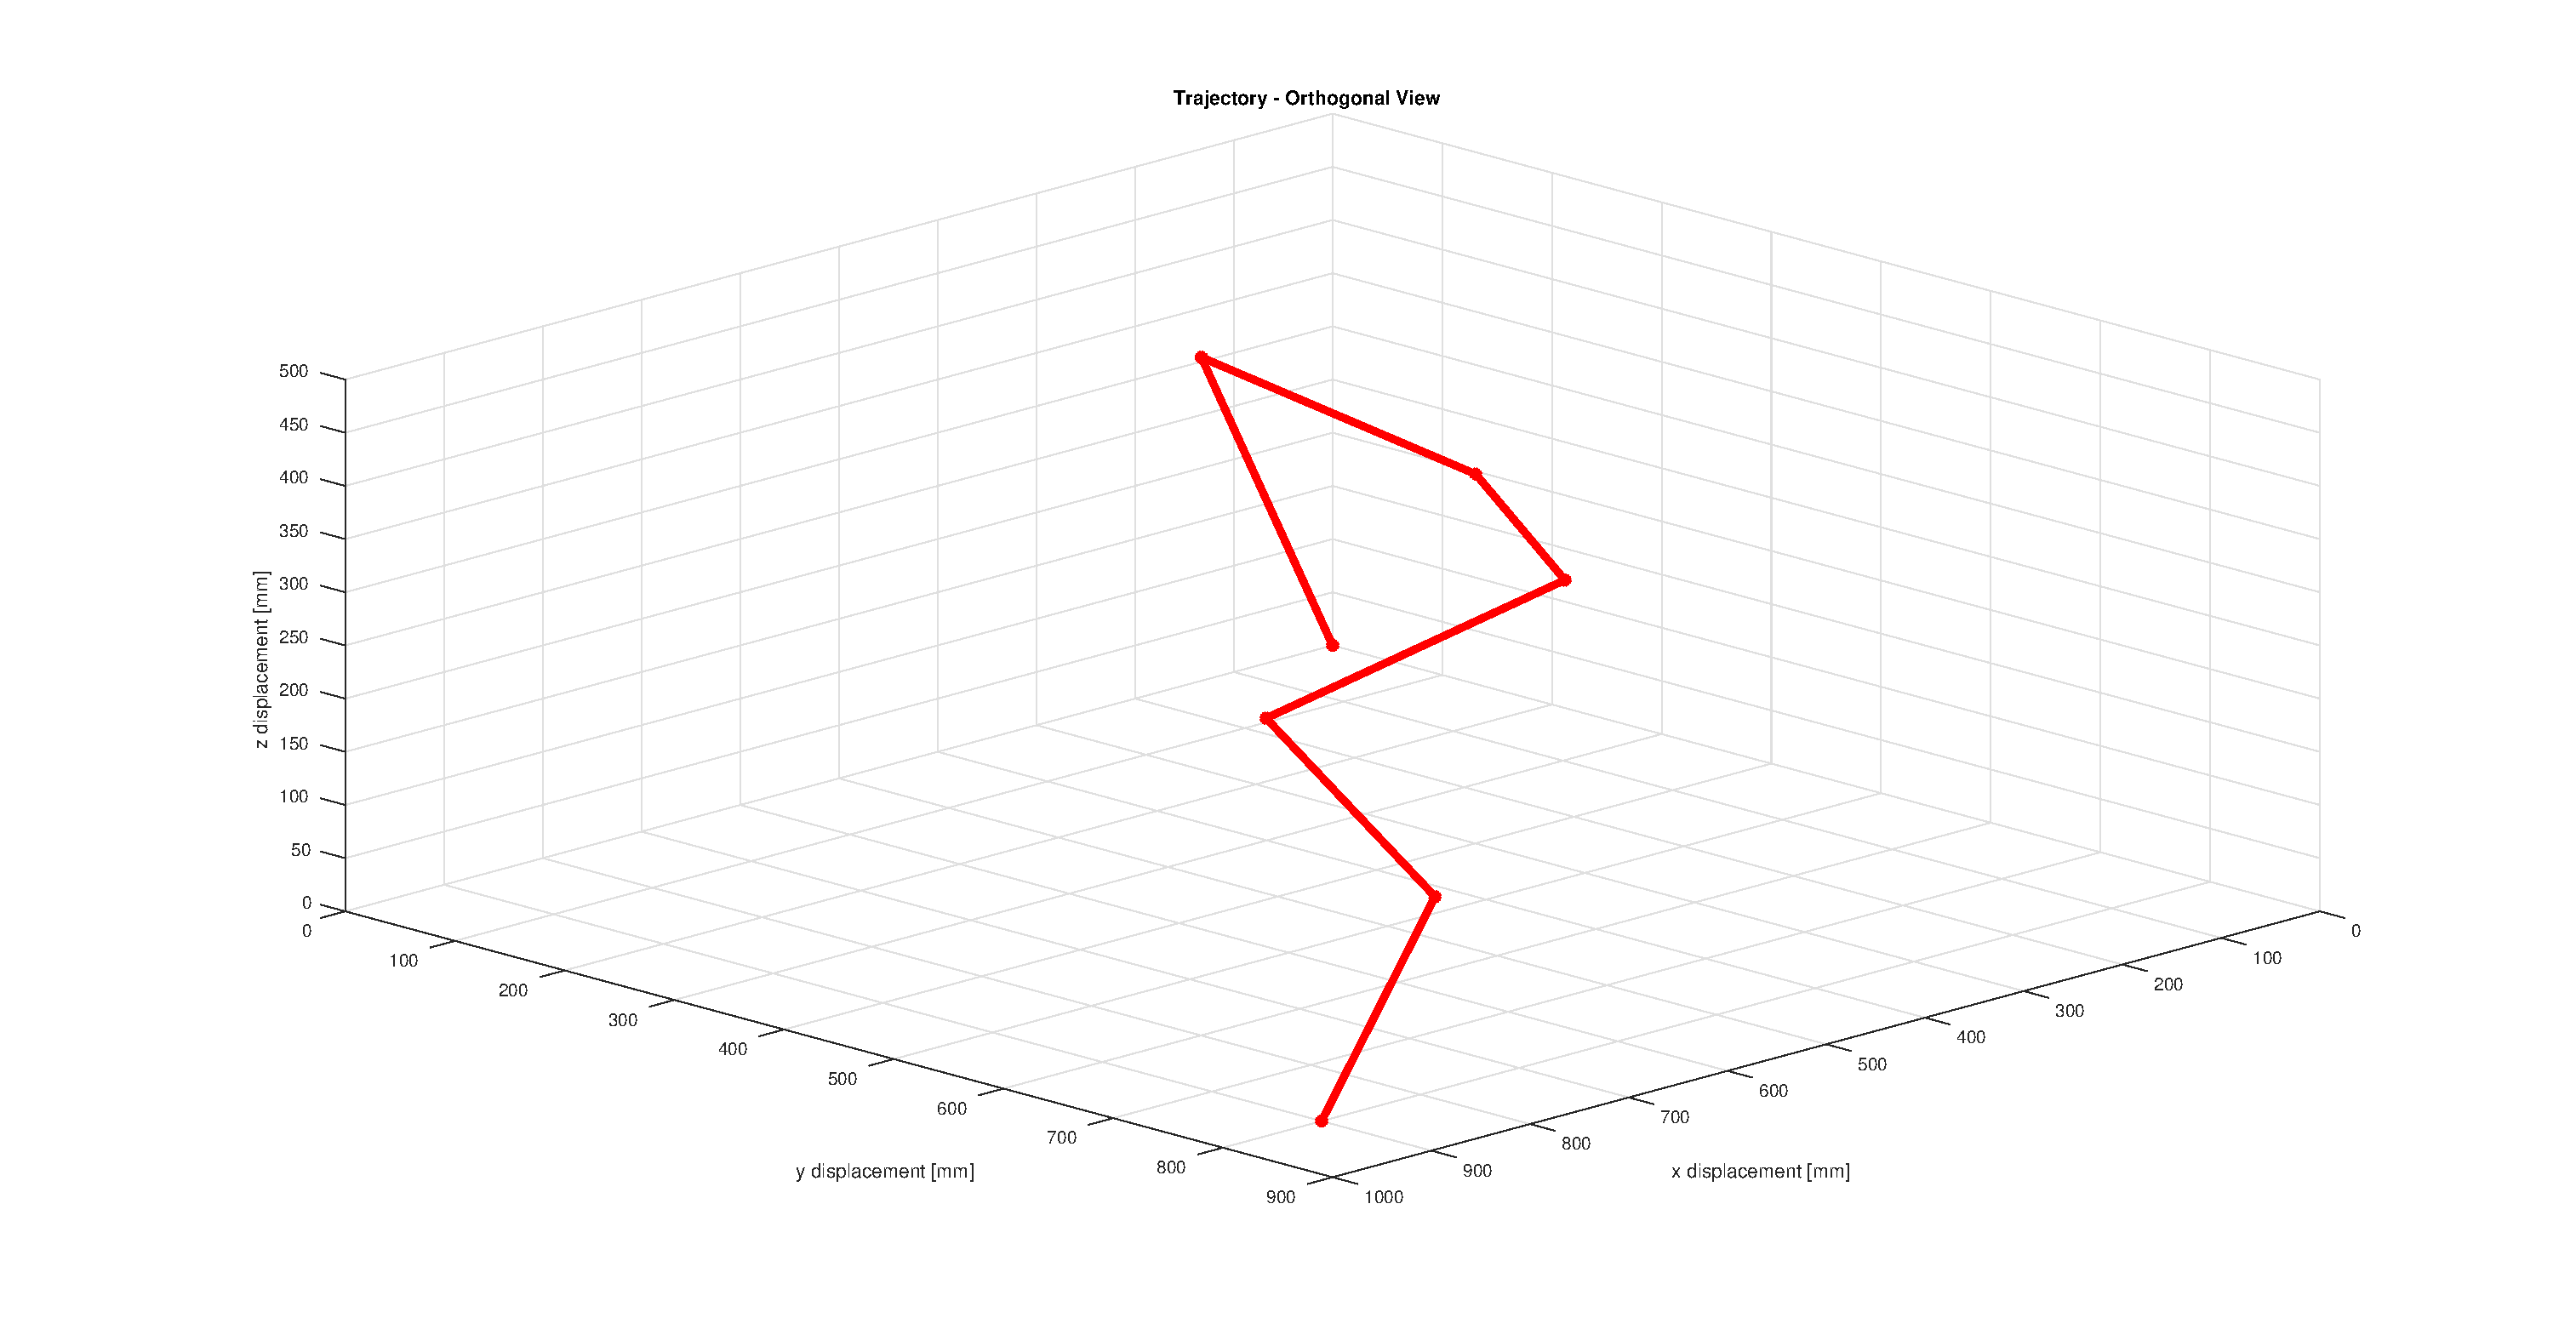
\includegraphics[height=0.45\linewidth, width=0.45\linewidth]{trajectory_no_simplify_orthogonal.eps}
	%		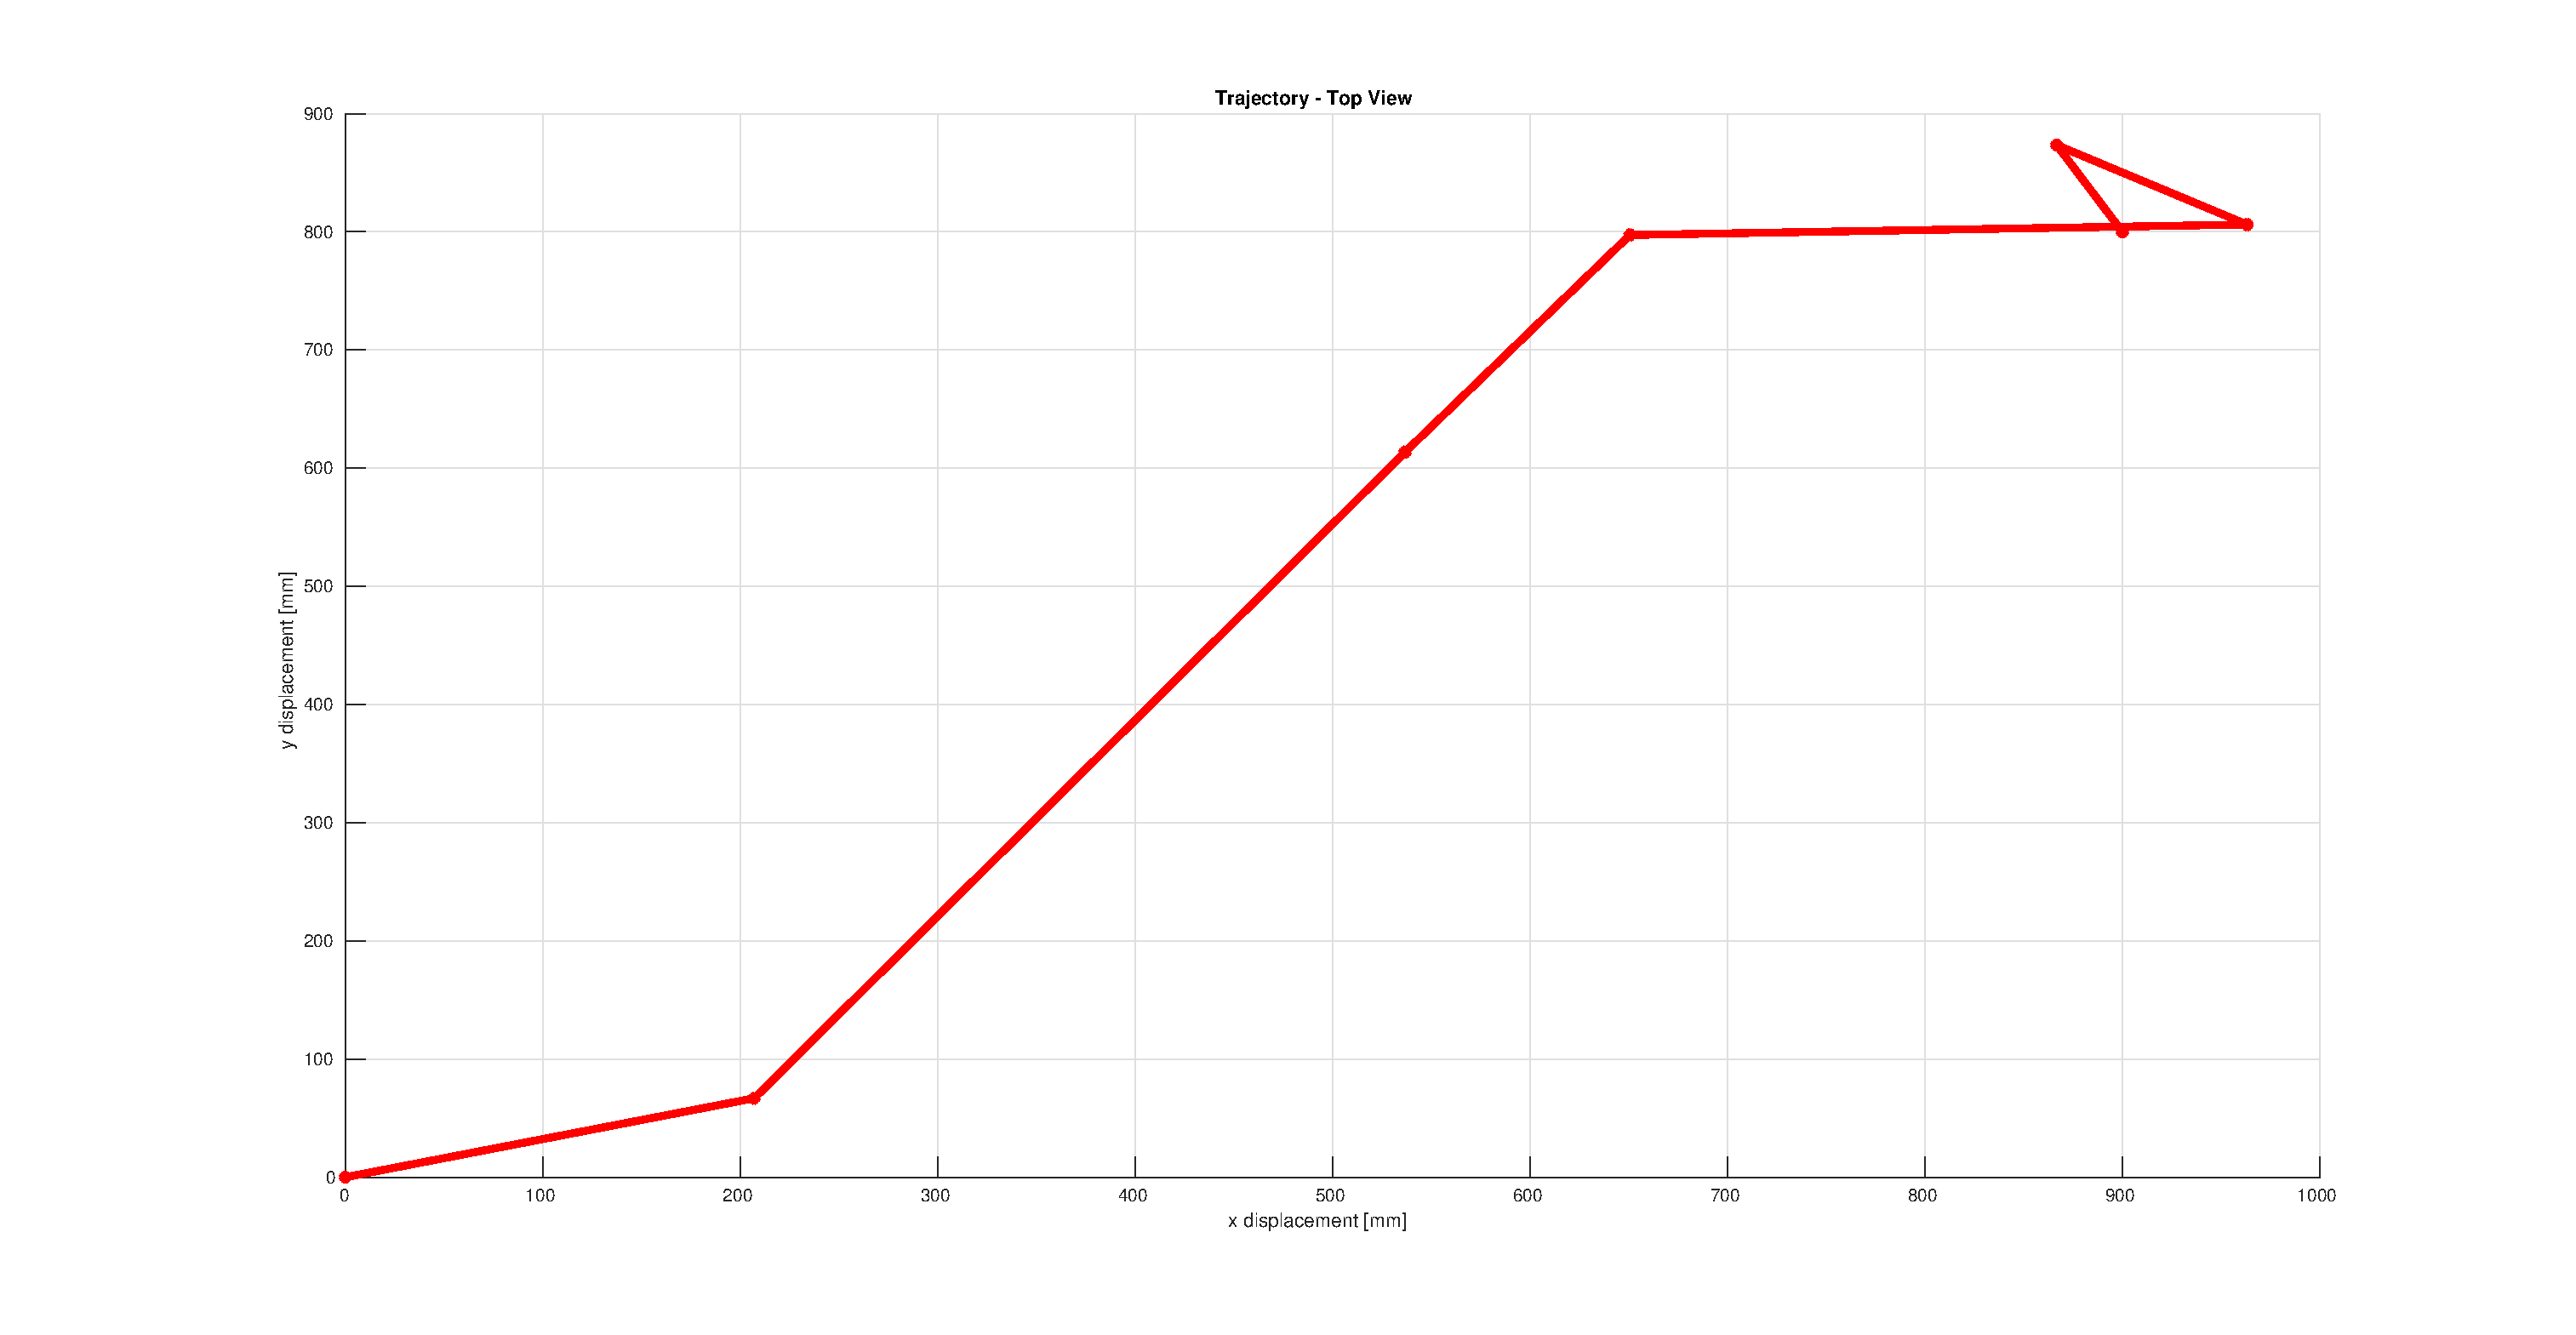
\includegraphics[height=0.45\linewidth, width=0.45\linewidth]{trajectory_no_simplify_top.eps}
	%	\end{minipage}
	%	\caption{Sample Trajectory Before Simplification}
	%\end{figure}

	\begin{figure}[hb]
		\centering
		\begin{minipage}{0.5\linewidth}
			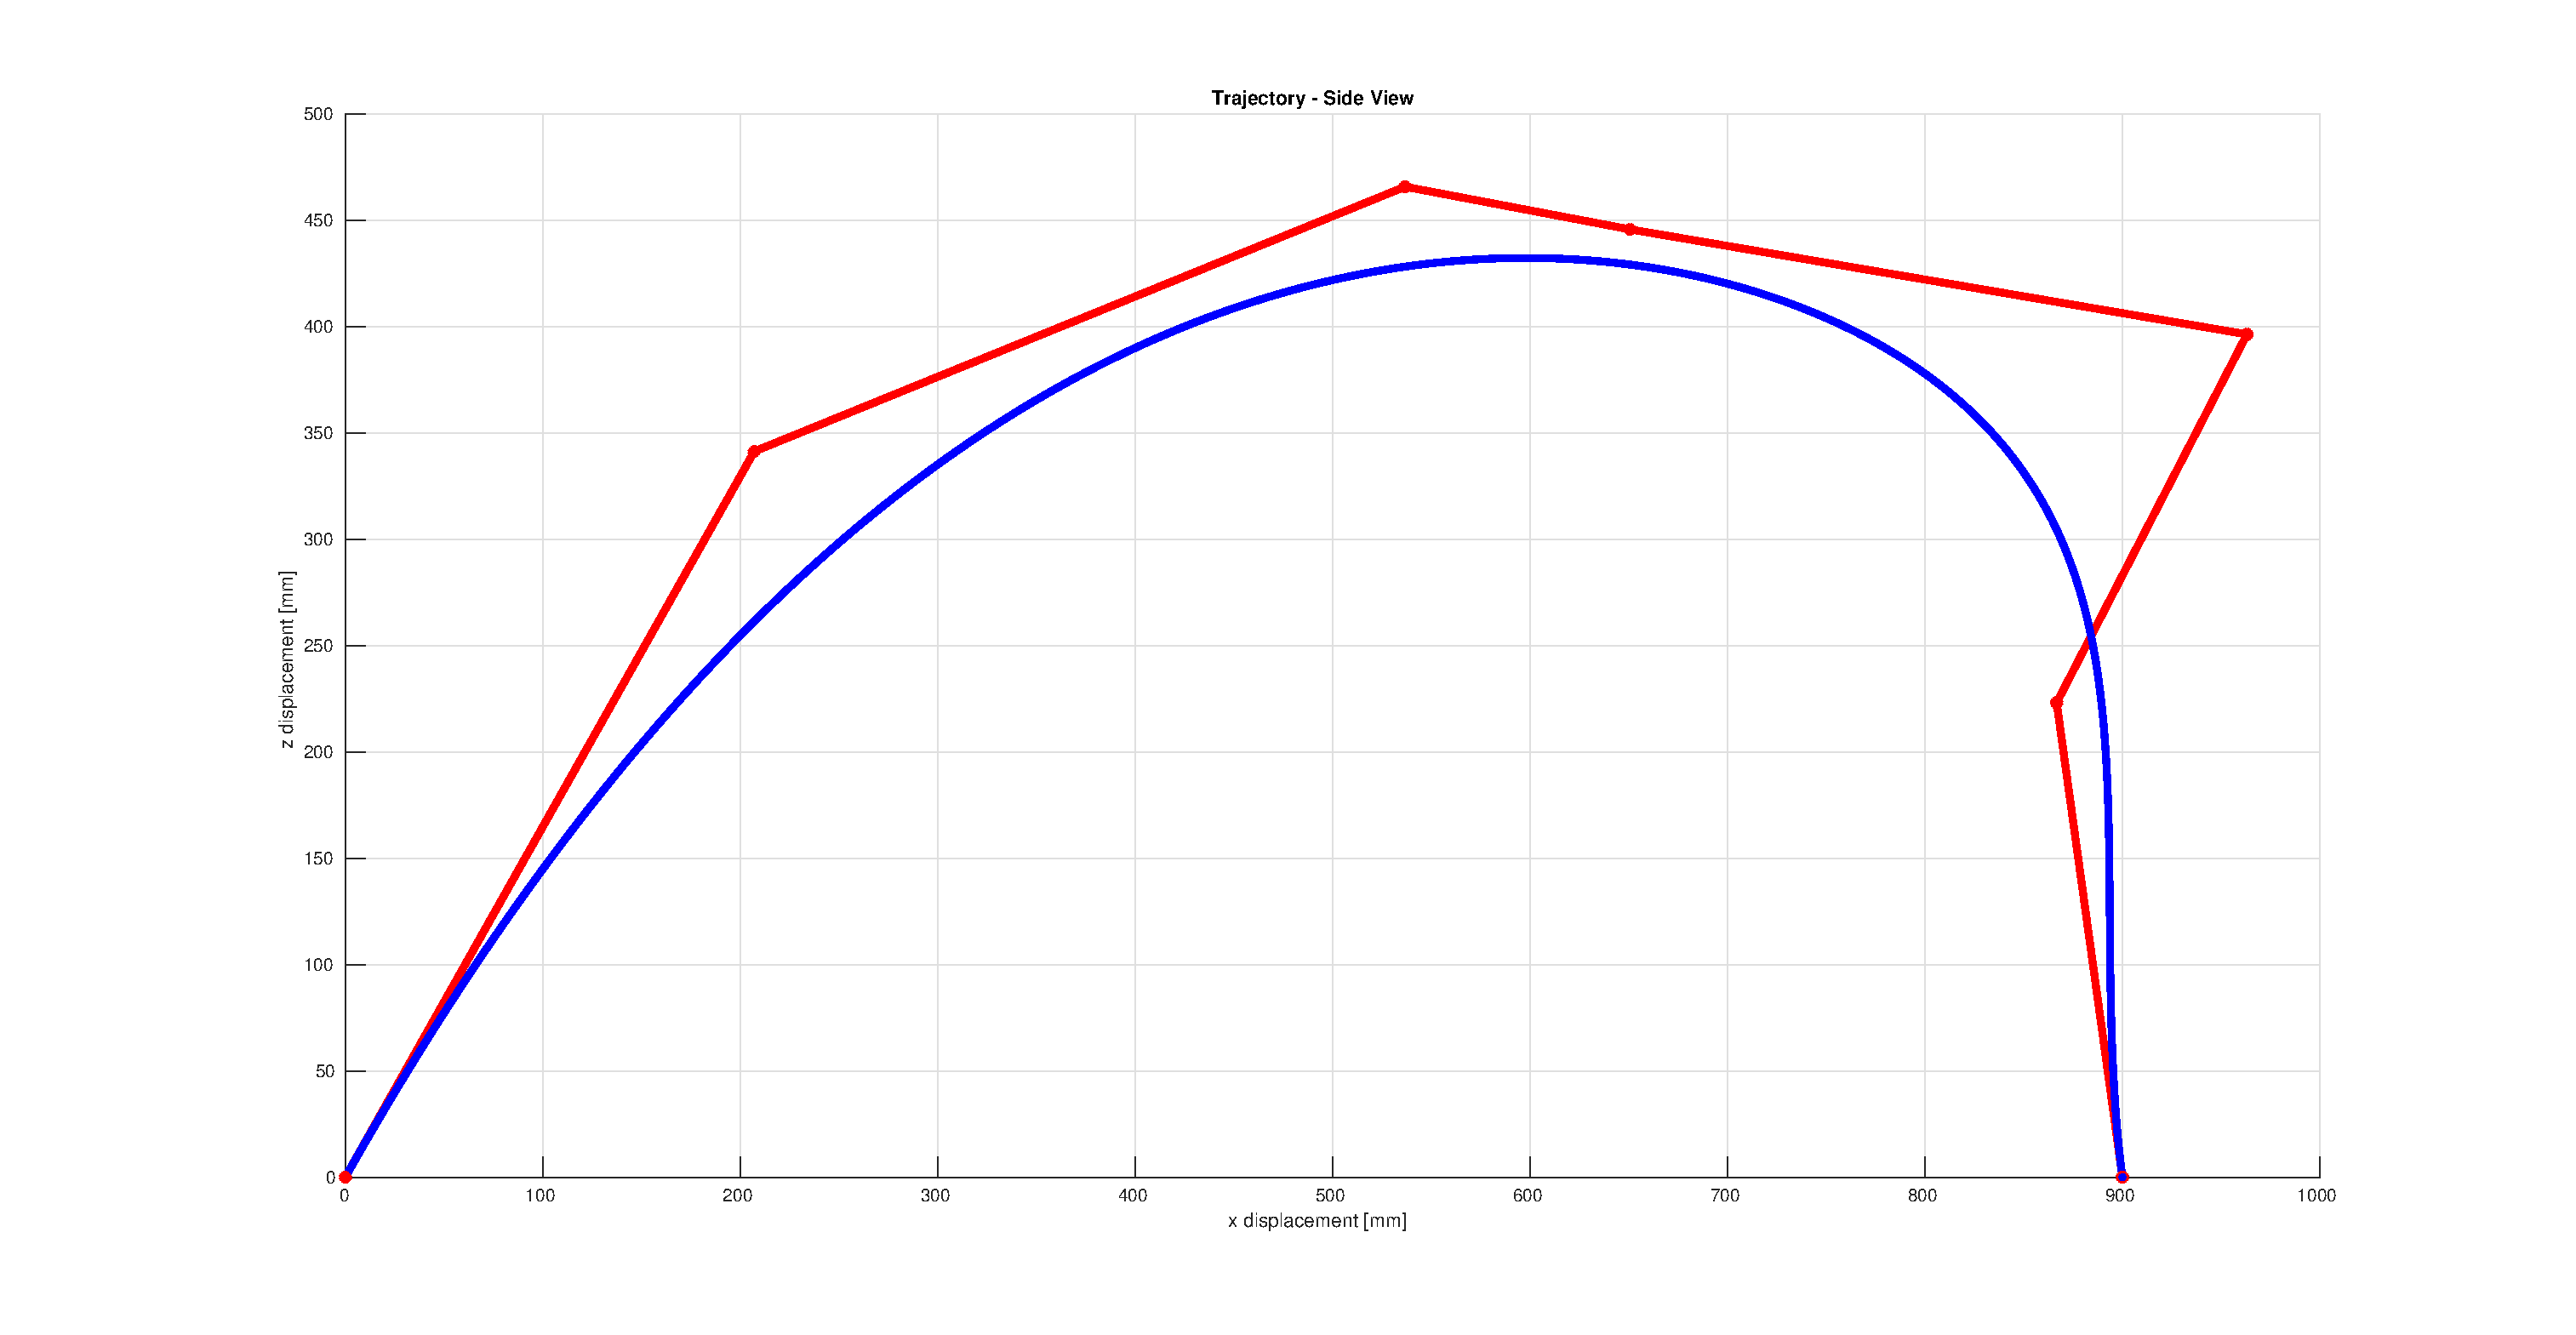
\includegraphics[height=0.45\linewidth, width=0.45\linewidth]{trajectory_simplify_no_subdivide_side.eps}
			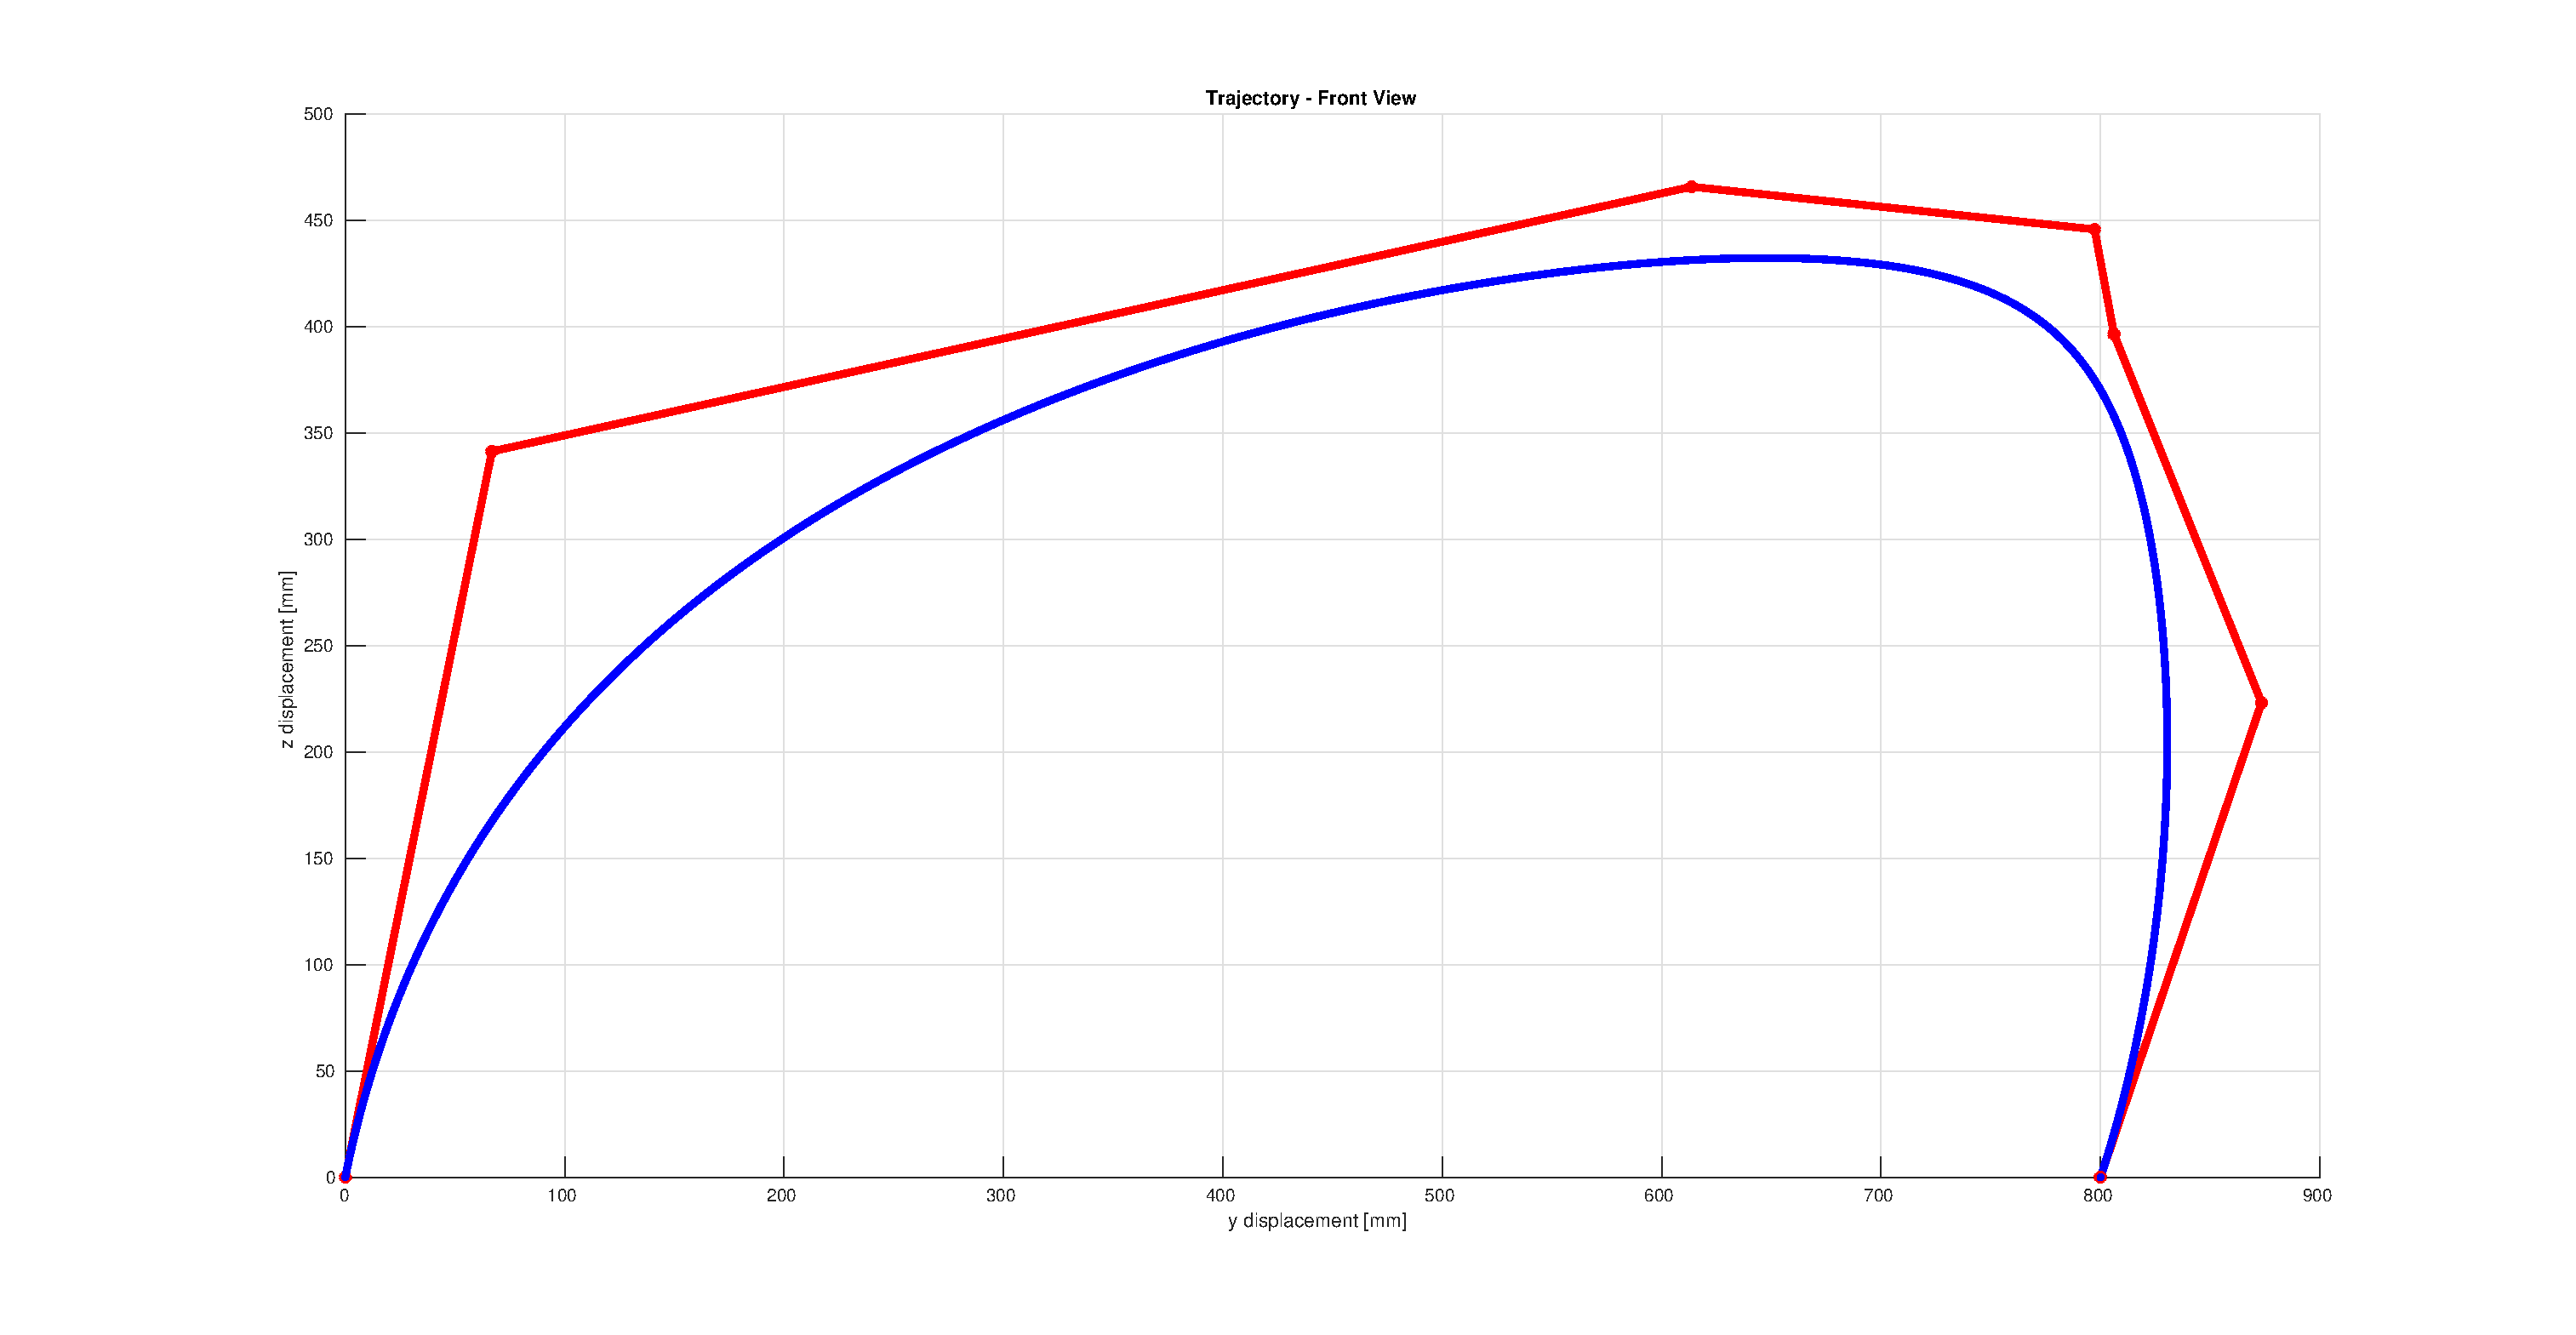
\includegraphics[height=0.45\linewidth, width=0.45\linewidth]{trajectory_simplify_no_subdivide_front.eps}
			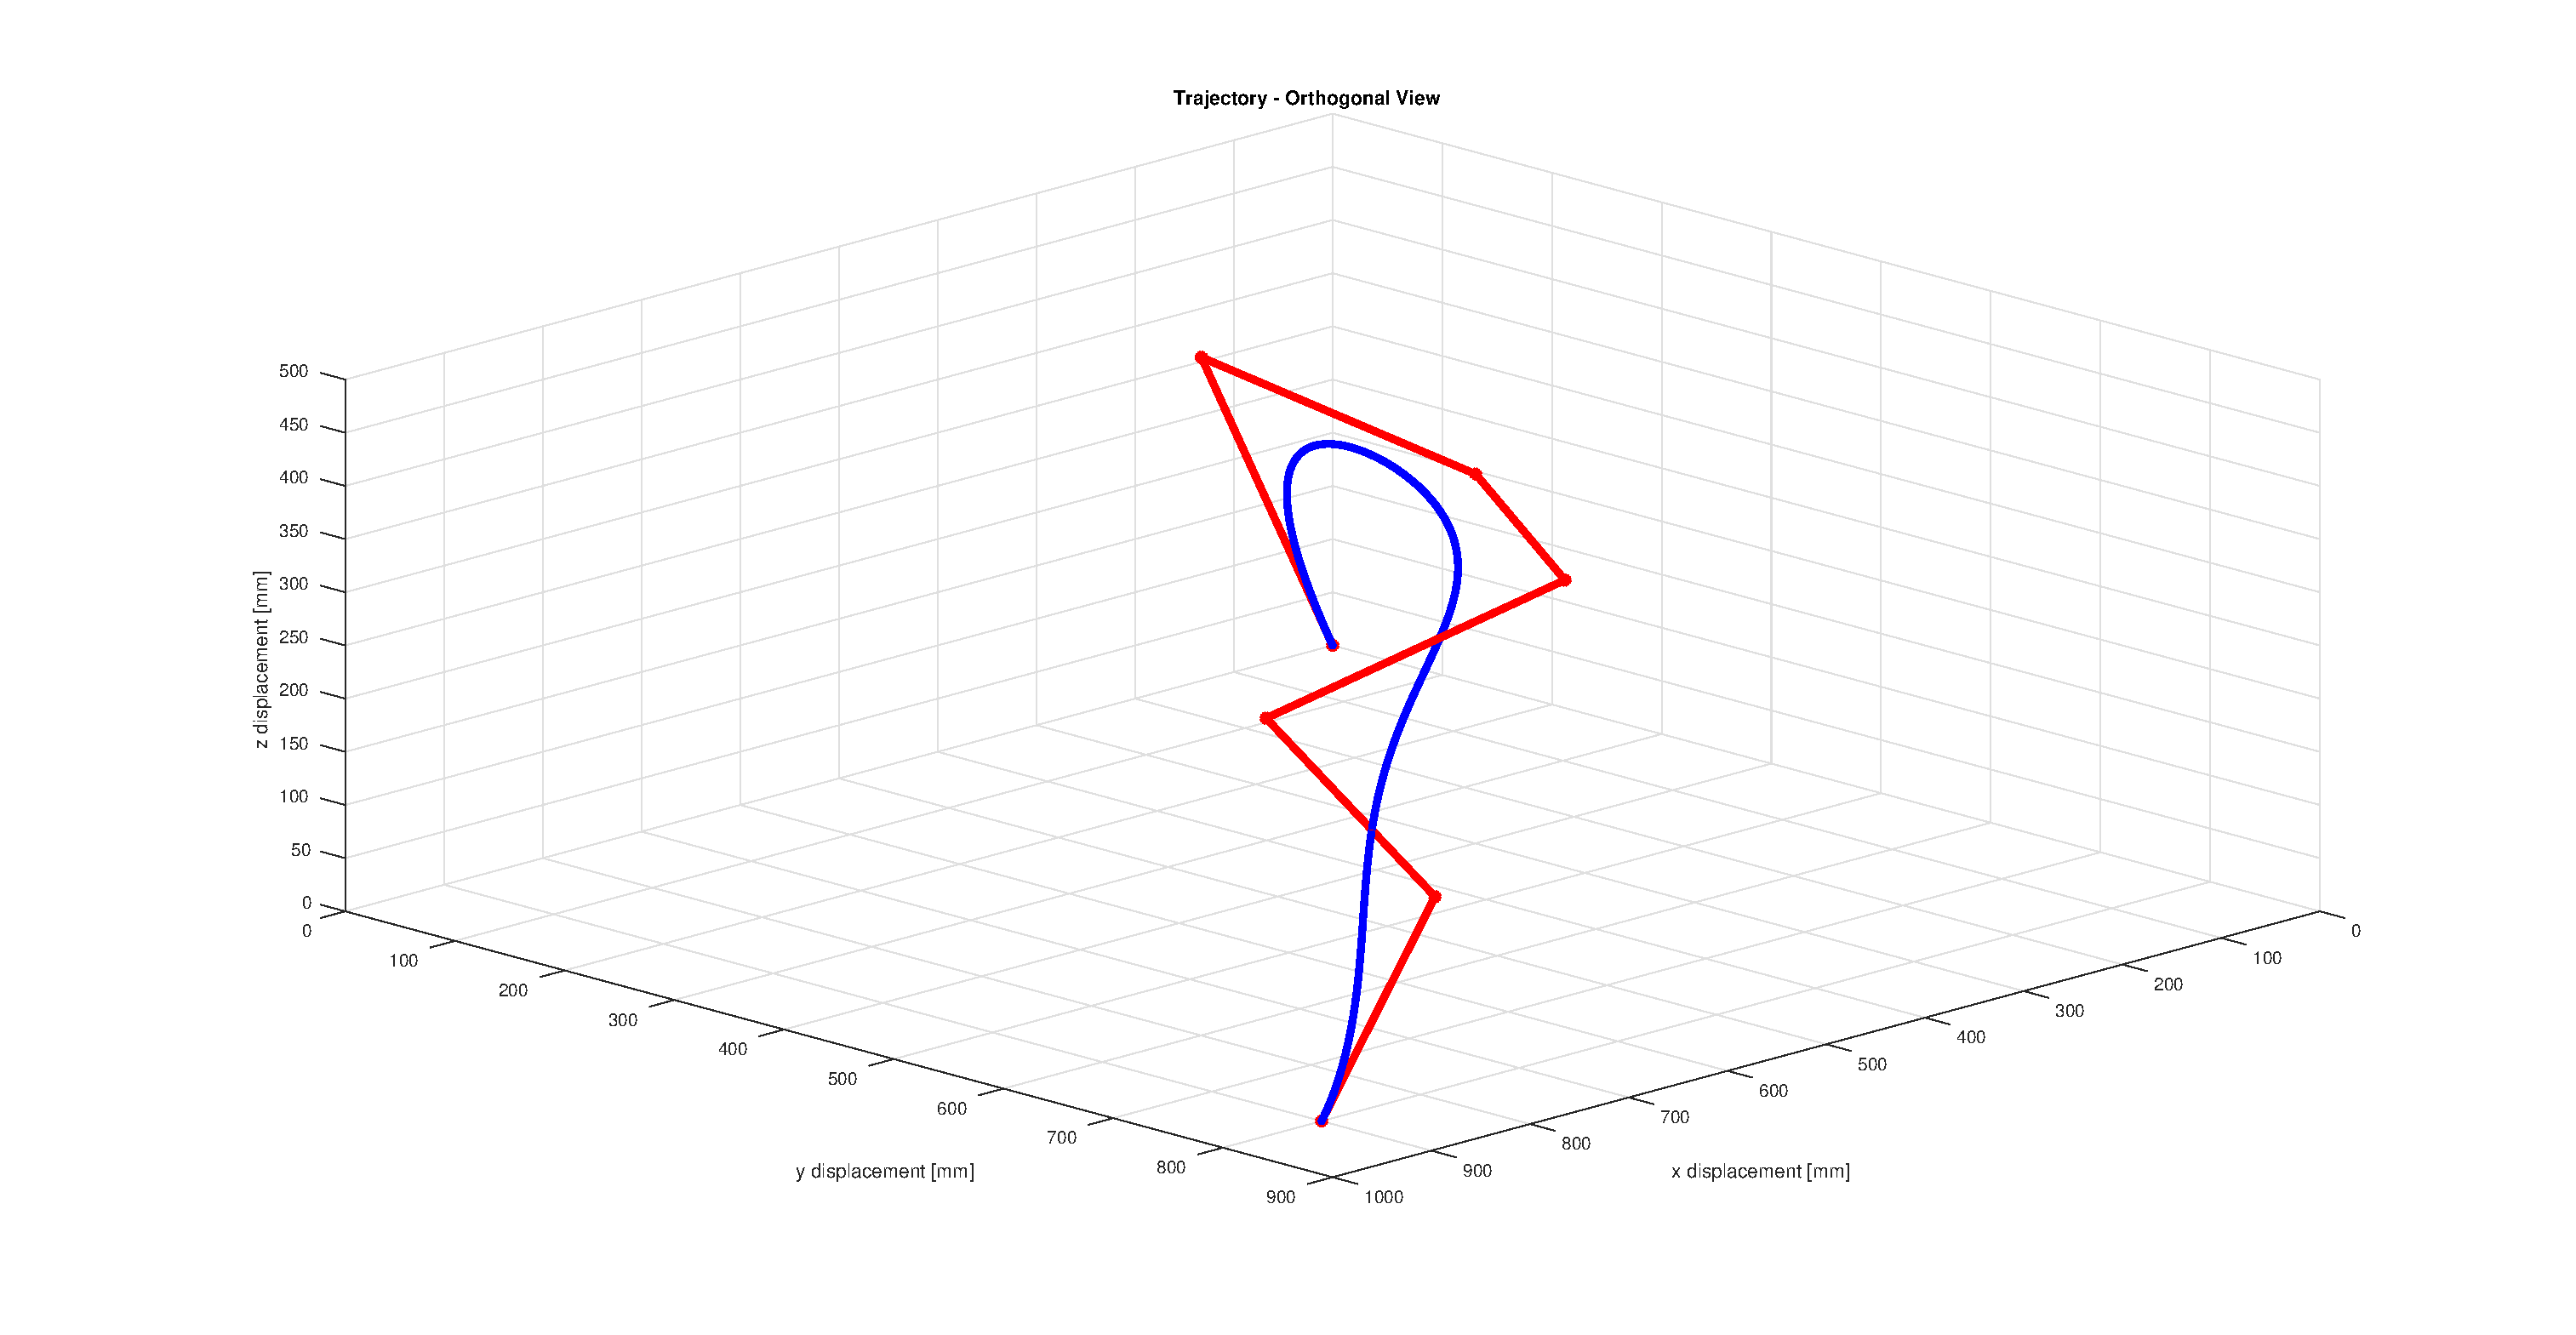
\includegraphics[height=0.45\linewidth, width=0.45\linewidth]{trajectory_simplify_no_subdivide_orthogonal.eps}
			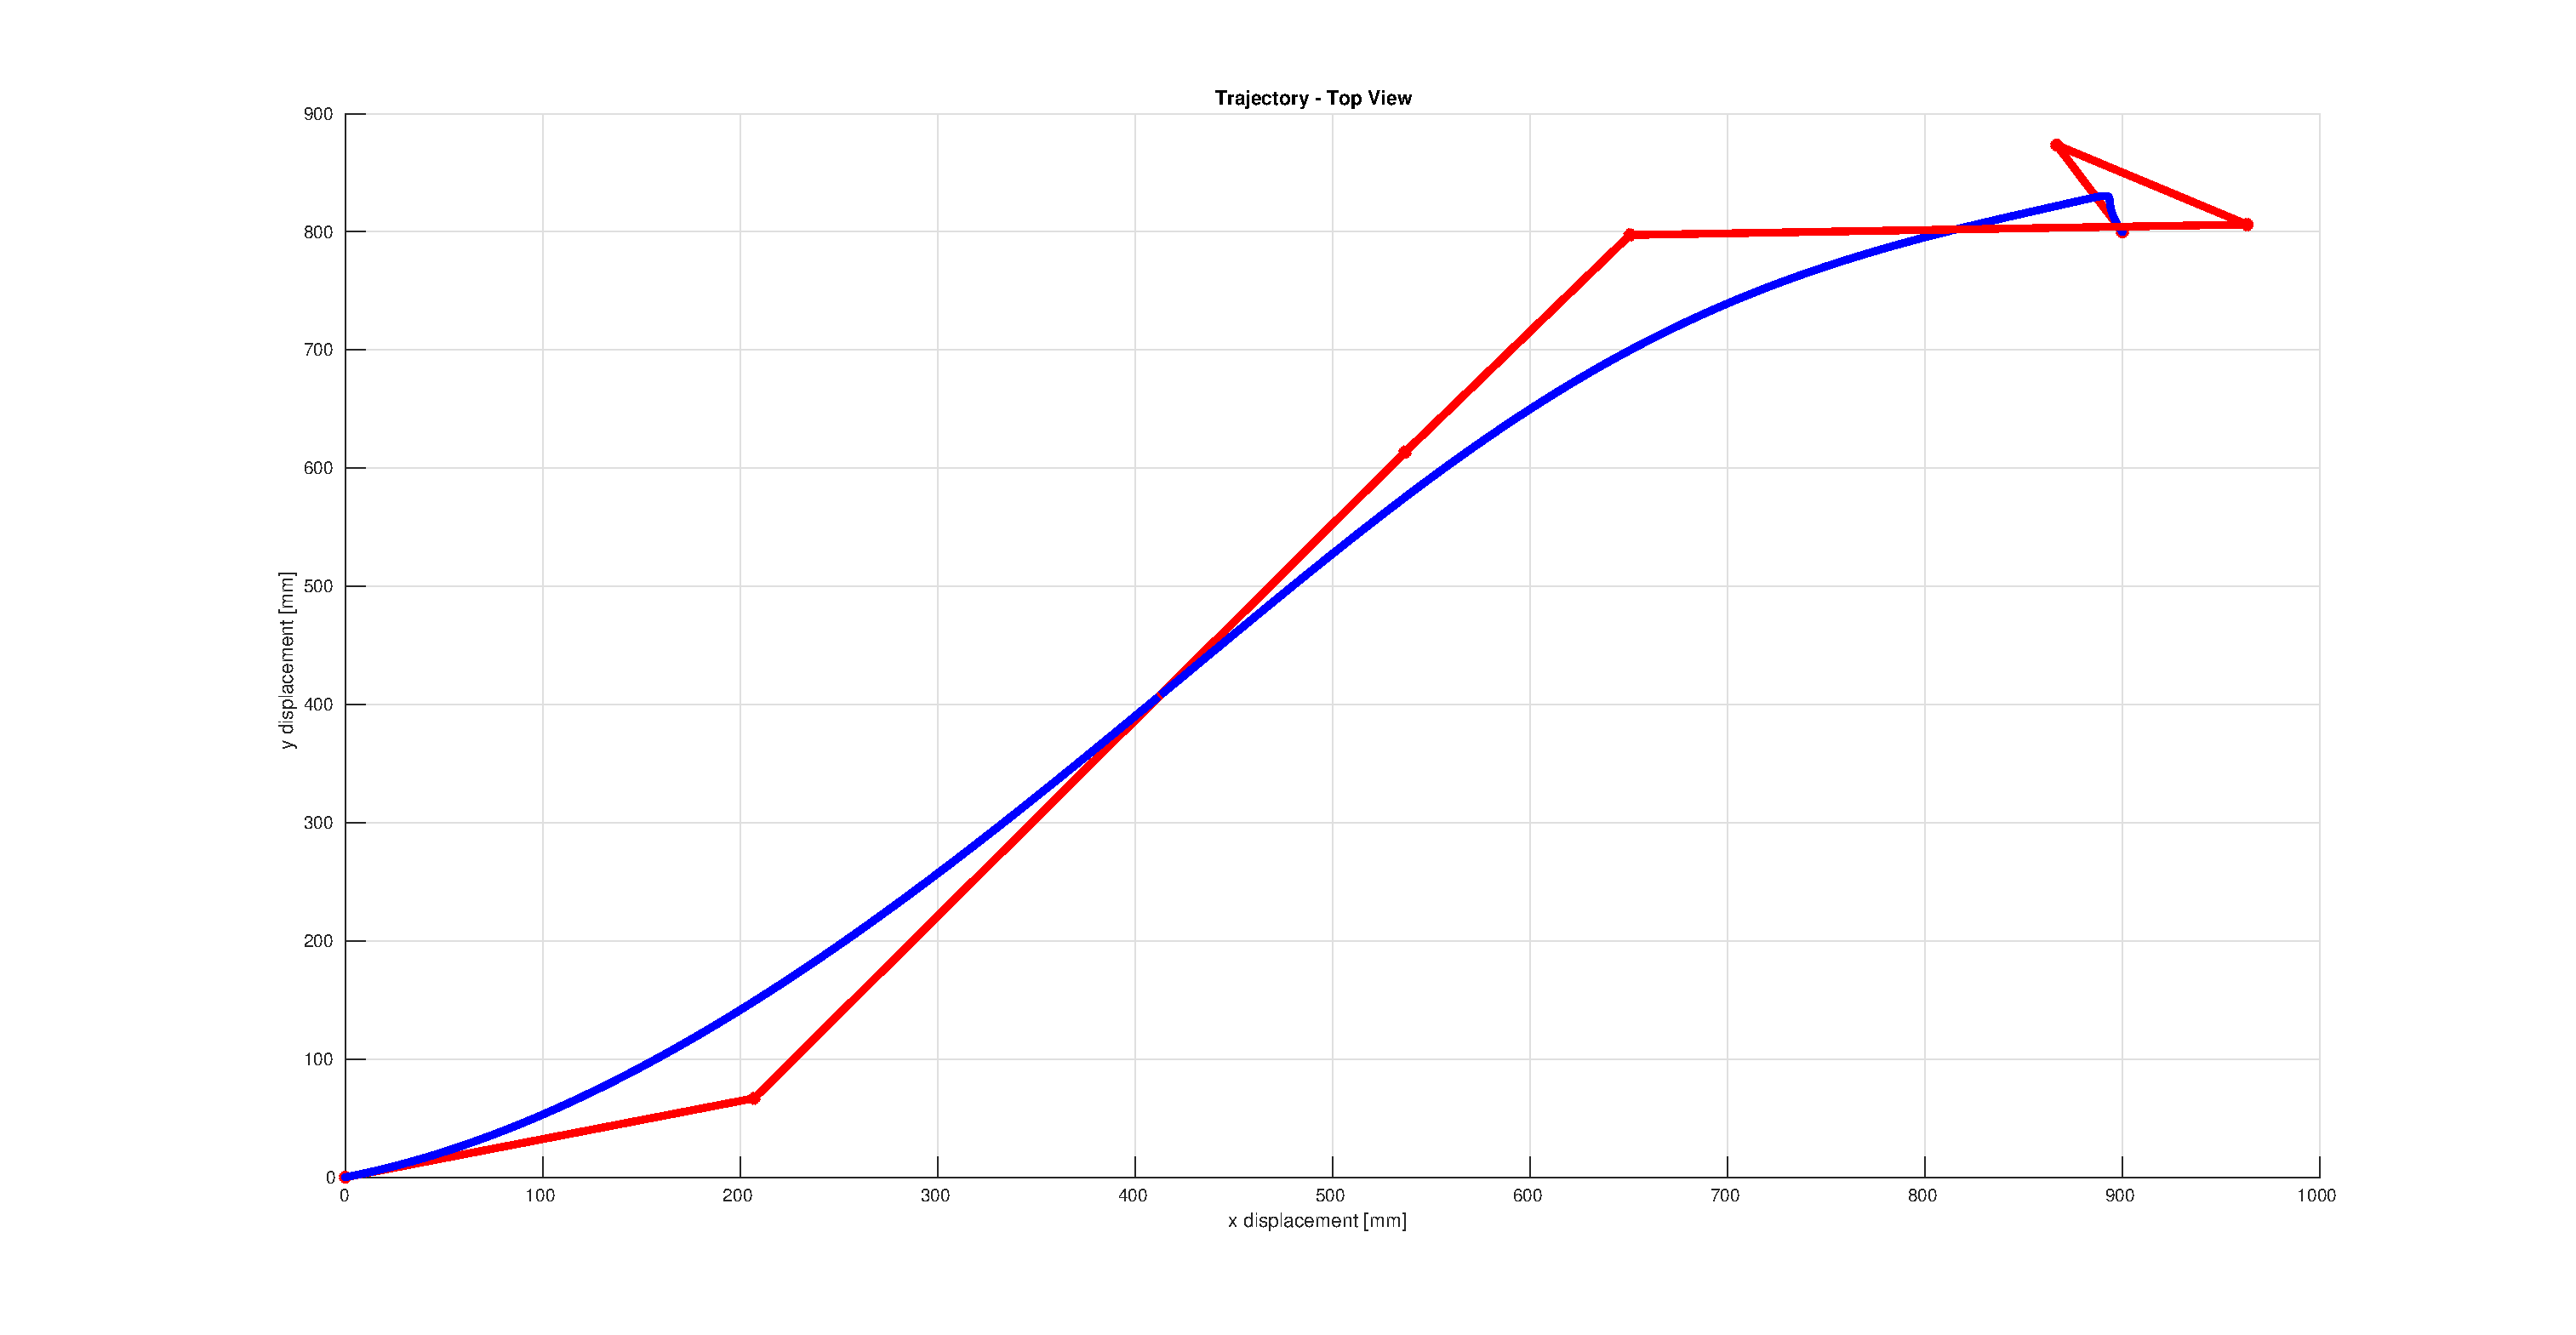
\includegraphics[height=0.45\linewidth, width=0.45\linewidth]{trajectory_simplify_no_subdivide_top.eps}
		\end{minipage}
		\caption{Sample Trajectory After Simplification}
		\label{fig:sample_trajectory_after_simplification}
	\end{figure}


	\begin{figure}[hb]
		\centering
		\begin{minipage}{0.5\linewidth}
			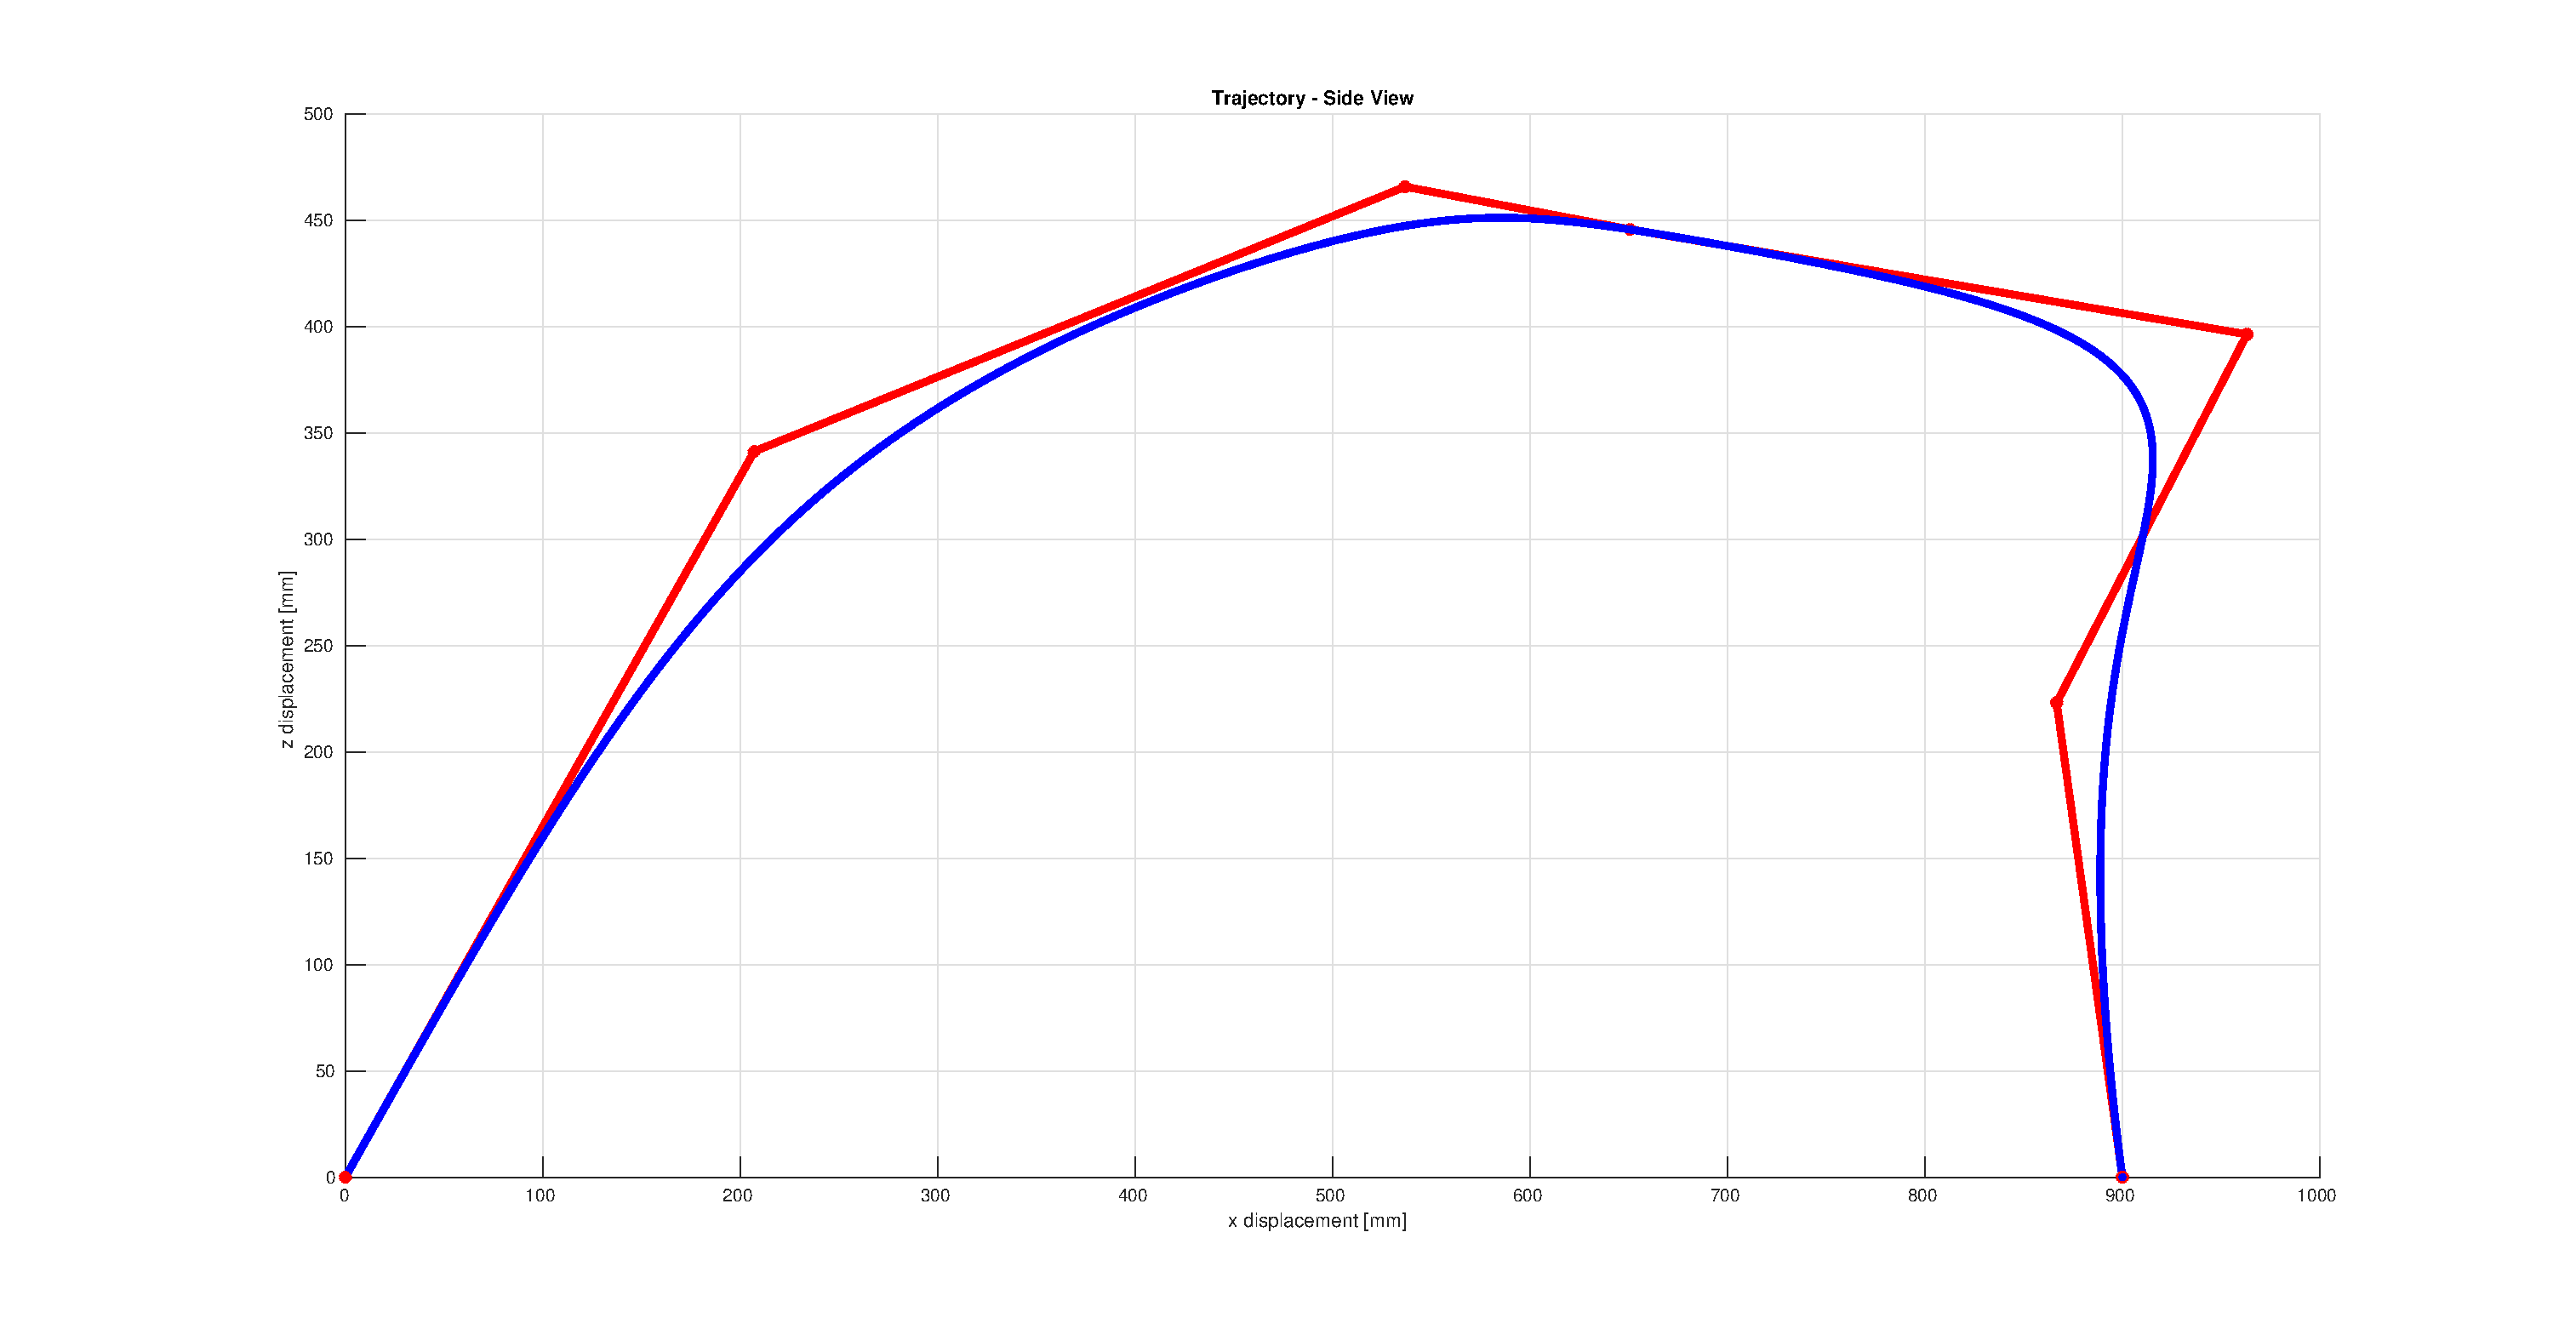
\includegraphics[height=0.45\linewidth, width=0.45\linewidth]{trajectory_simplify_subdivide_side.eps}
			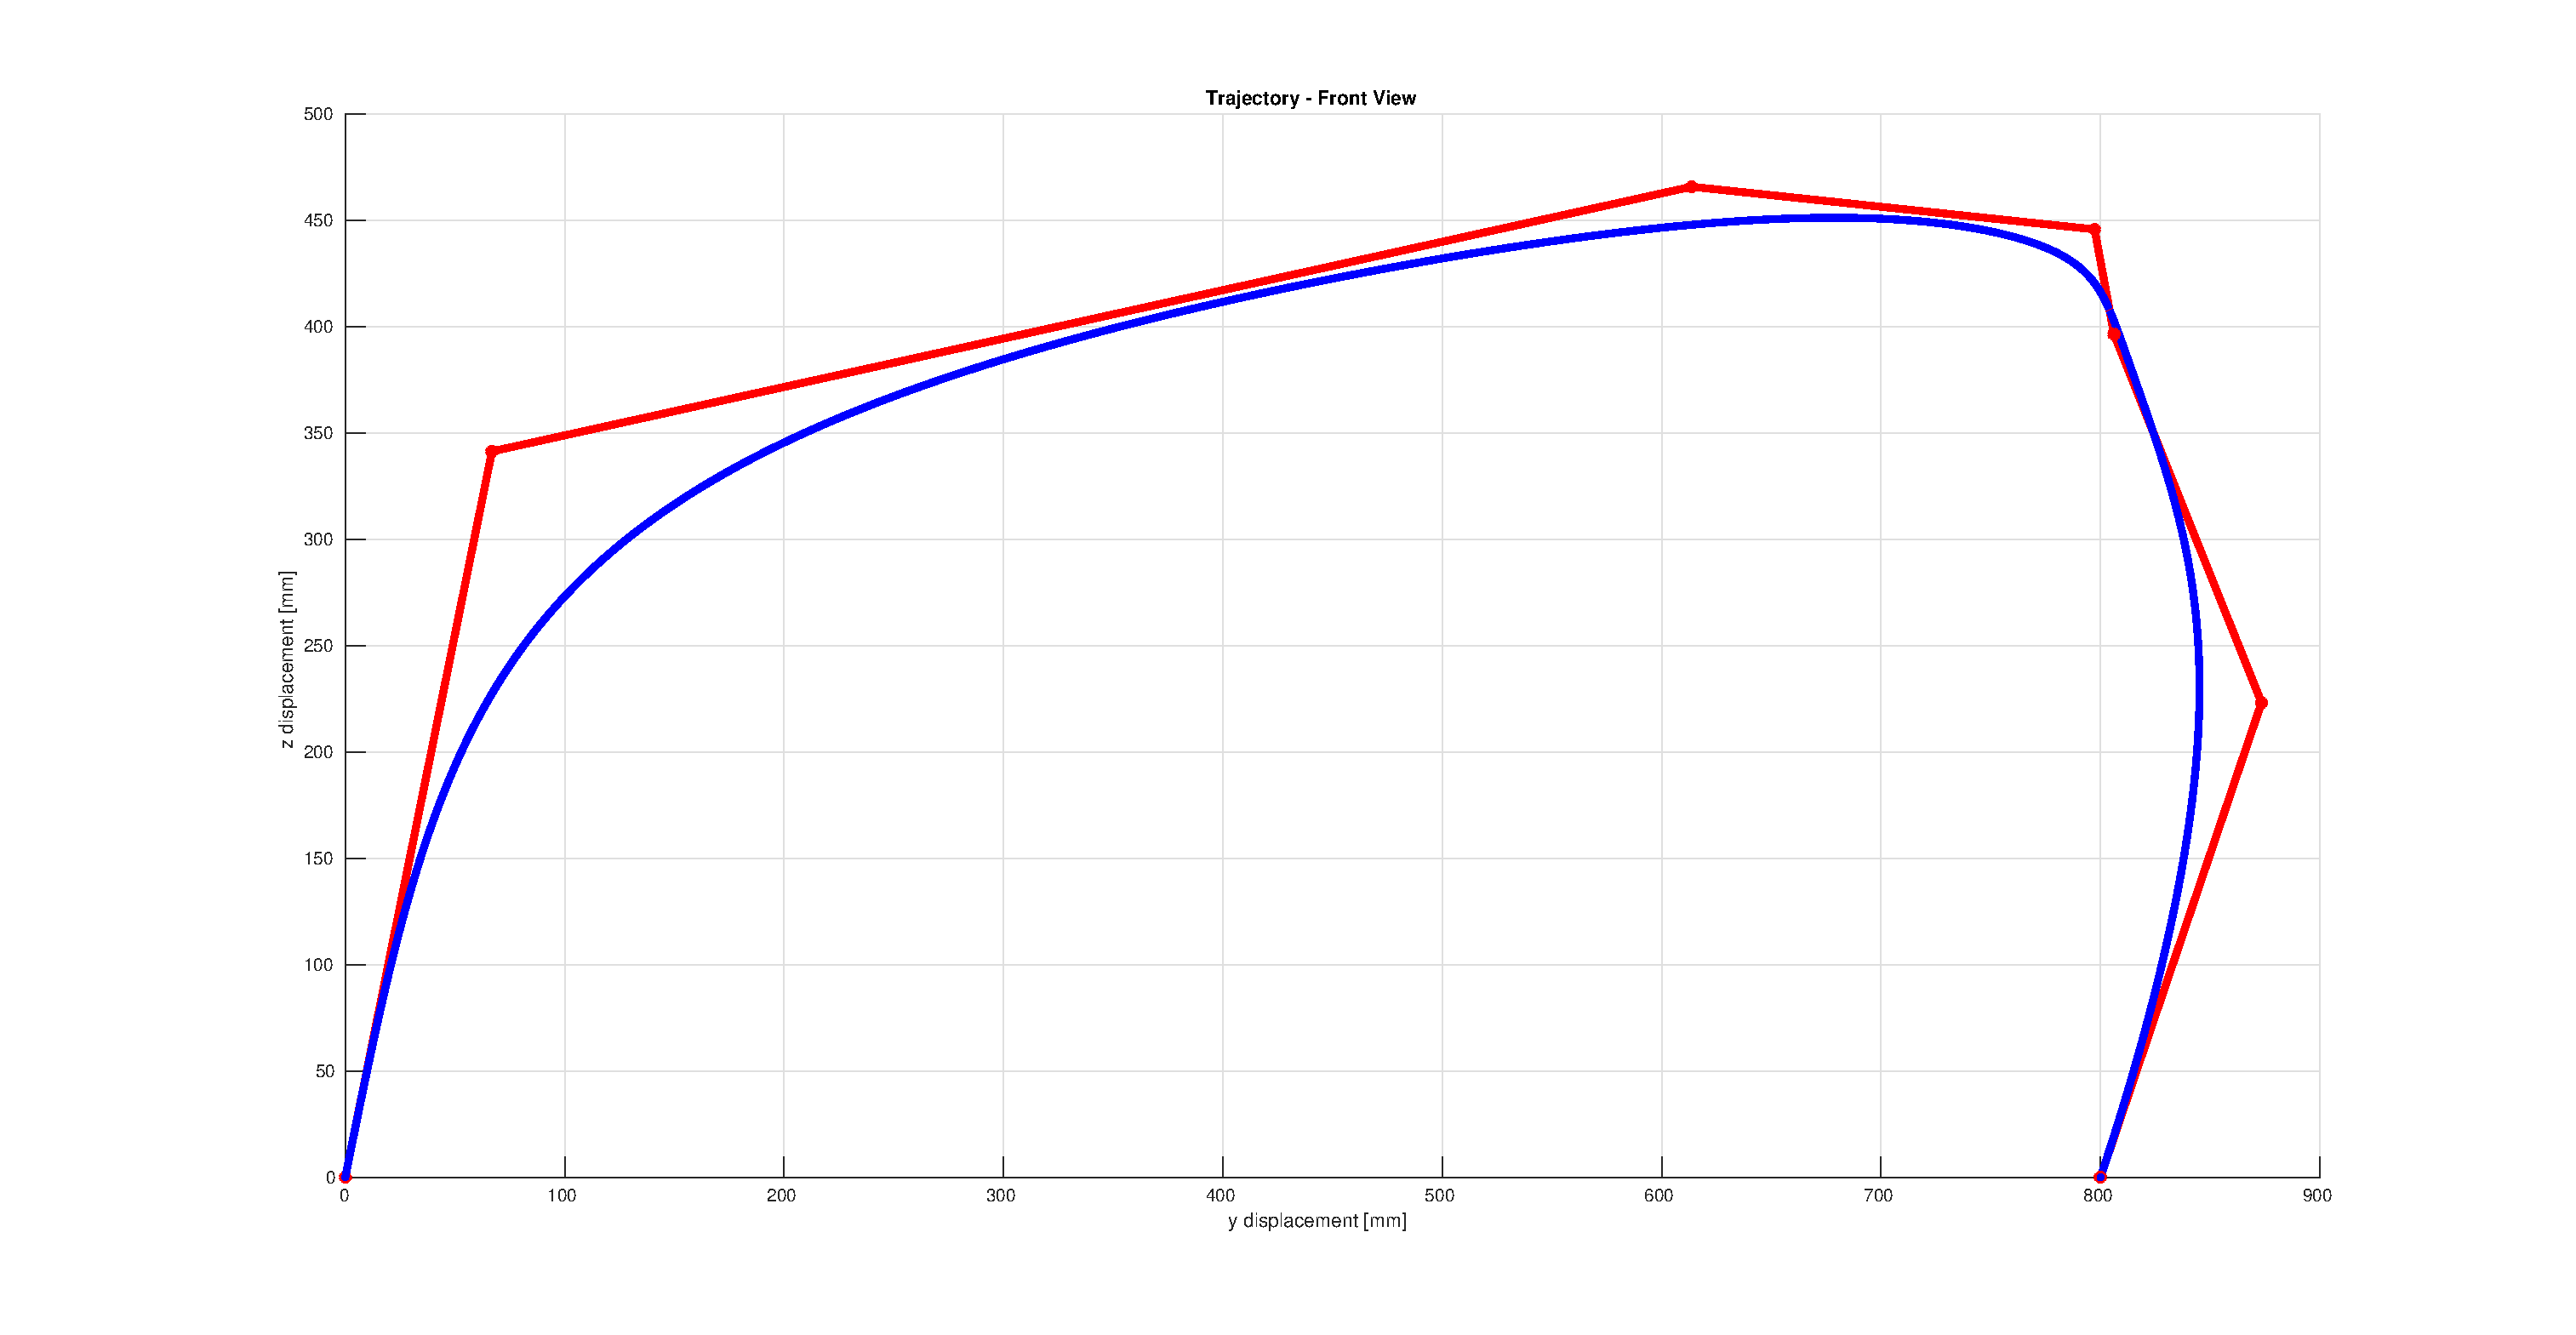
\includegraphics[height=0.45\linewidth, width=0.45\linewidth]{trajectory_simplify_subdivide_front.eps}
			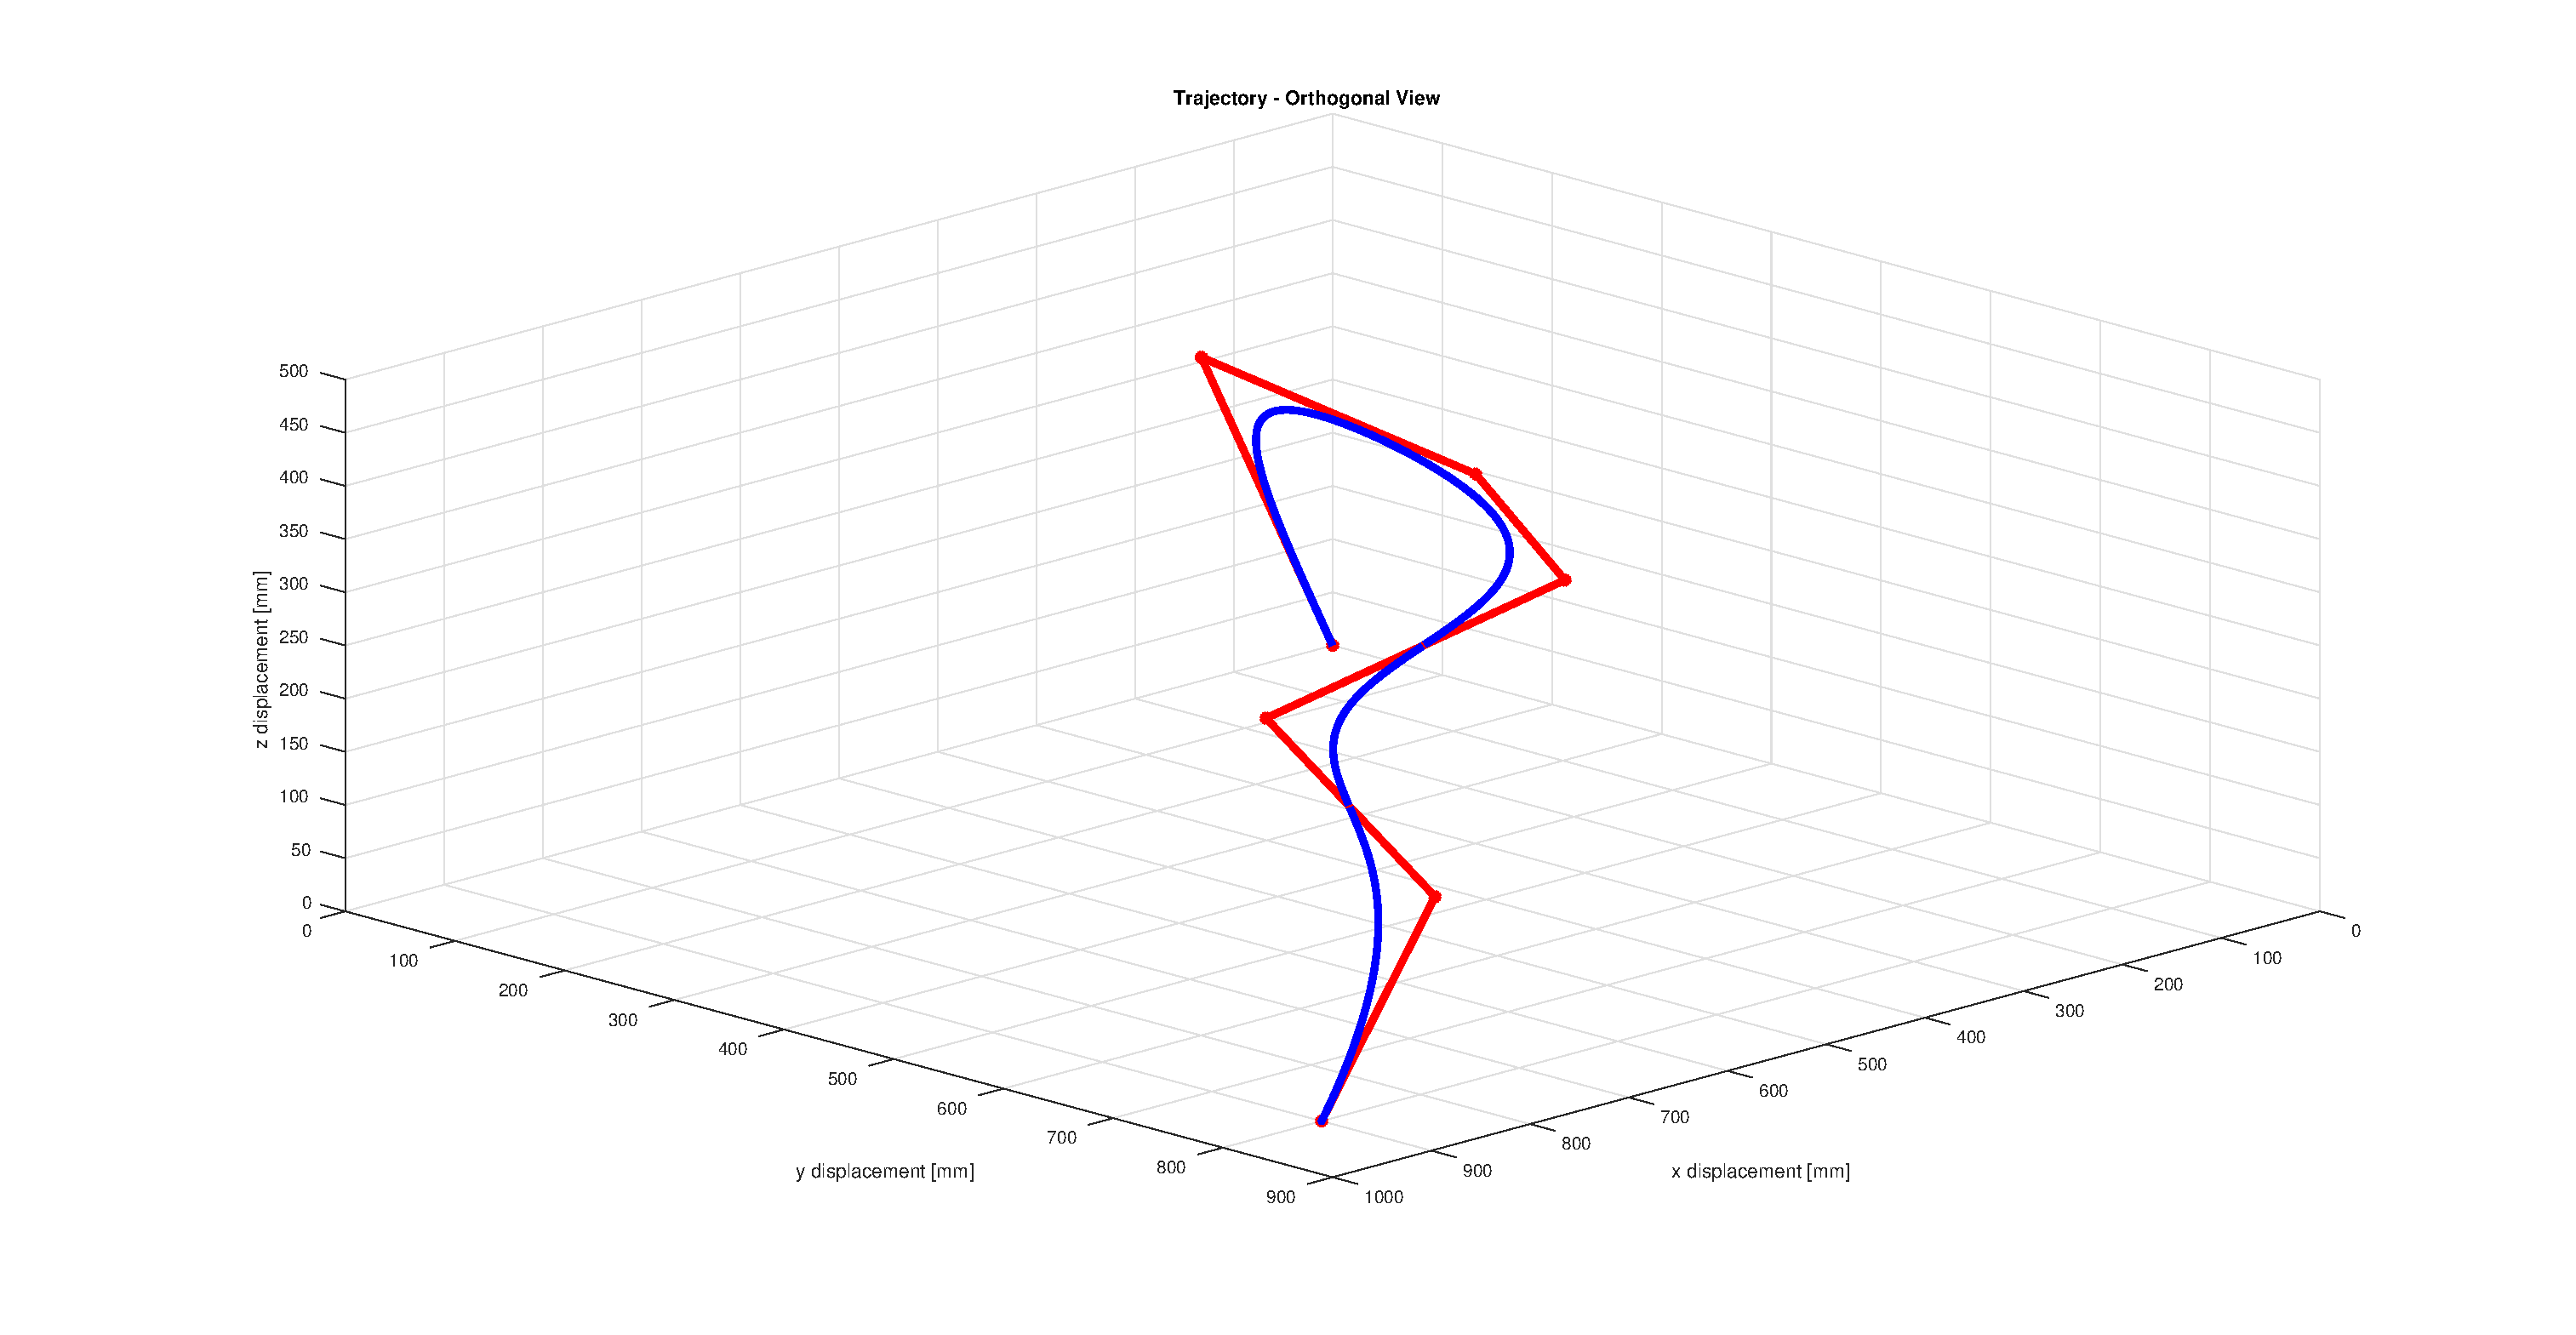
\includegraphics[height=0.45\linewidth, width=0.45\linewidth]{trajectory_simplify_subdivide_orthogonal.eps}
			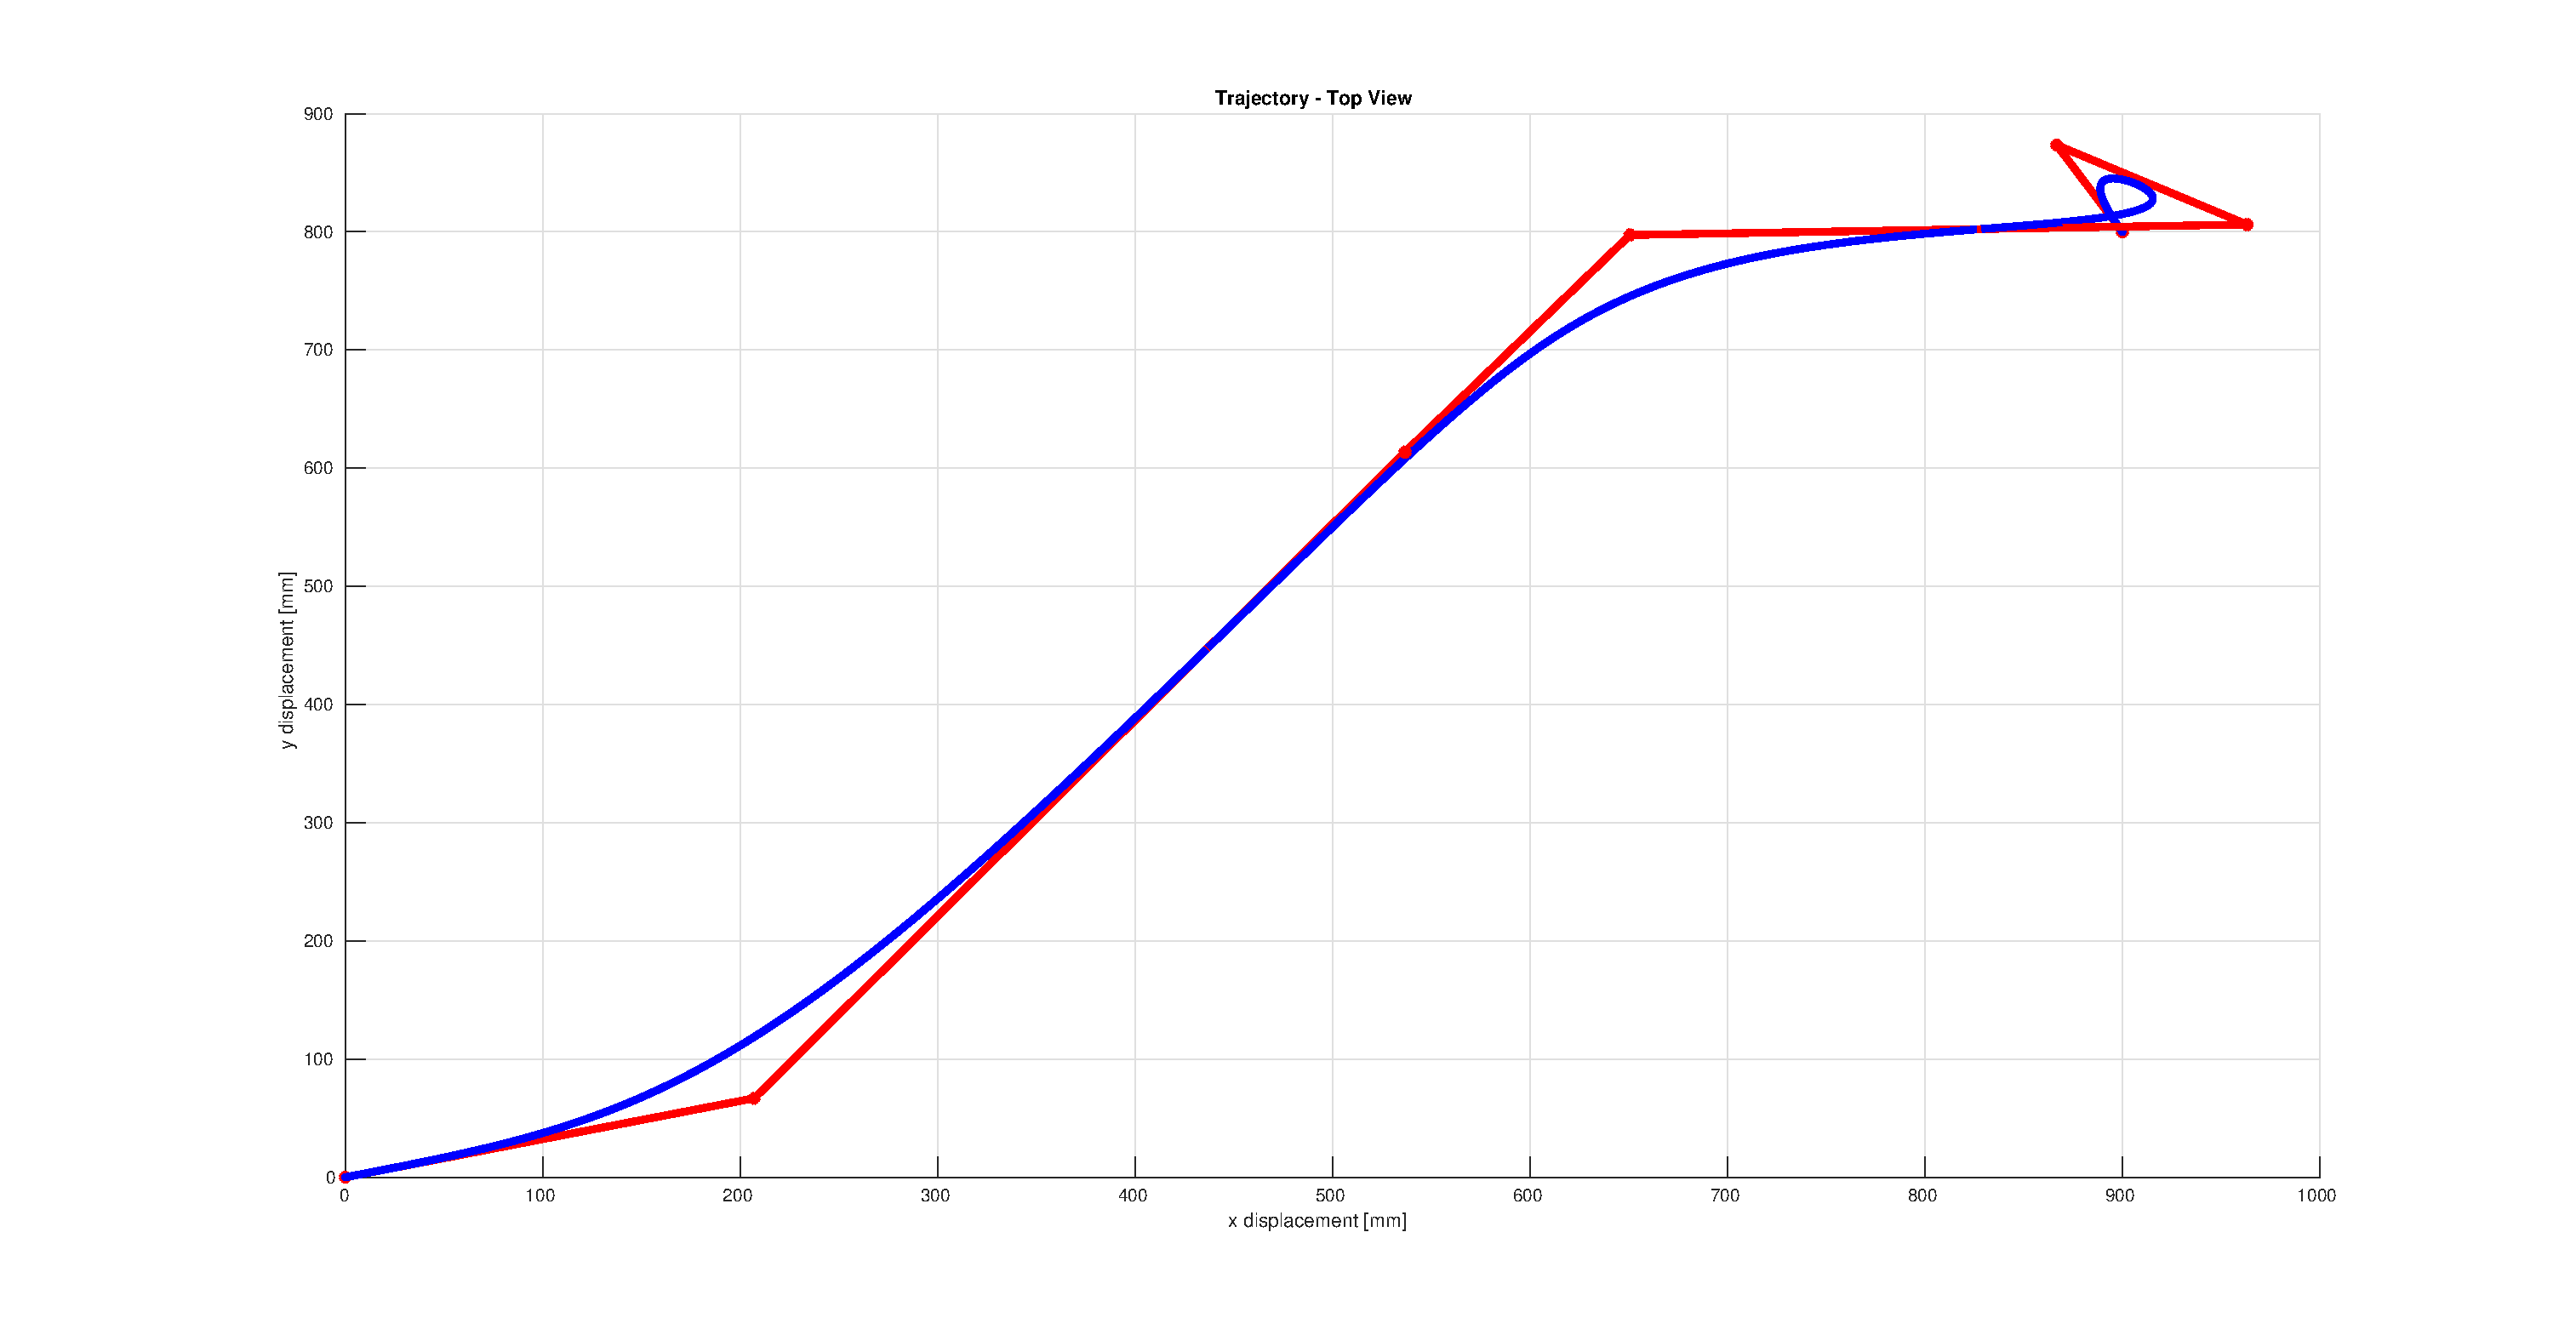
\includegraphics[height=0.45\linewidth, width=0.45\linewidth]{trajectory_simplify_subdivide_top.eps}
		\end{minipage}
		\caption{Sample Trajectory with Augmented $\setofposes$}
		\label{fig:sample_trajectory_with_augmented_set_of_poses}
	\end{figure}

	The figures show, in order, the right, front, orthogonal and top views of
	the trajectory. The red straight lines represent the path found in the
	topological graph after the path simplification algorithms of
	Section~\ref{sec:path_simplification} have been run. These lines are
	guaranteed to be free of collisions by the path-planning algorithms in
	Chapter~\ref{chap:sampling}.

	The smooth line in Figure~\ref{fig:sample_trajectory_after_simplification}
	shows what the trajectory would look like if
	Algorithm~\ref{alg:set_of_poses_augmentation} were not run. Note especially
	how, in the orthogonal view, the trajectory can be seen to completely ignore
	the corner in the front. This issue is aggravated when trajectories of a
	higher degree of smoothness are required. Higher-degree B-spline curves'
	tendency to seemingly `ignore' a control point can lead to large deviations
	from the path guaranteed in $\topologicalgraph$ and can hence lead to
	collisions.

	Figure~\ref{fig:sample_trajectory_with_augmented_set_of_poses} shows the
	effect of instead running Algorithm~\ref{alg:set_of_poses_augmentation} on
	$\setofposes$ found from $\topologicalgraph$. Note from the orthogonal view
	that the trajectory now comes much closer to the corner, yet is still able
	to keep the requested degree of smoothness. One can also note that the
	trajectory stays much closer to the control polygon. From the top and side
	views it is clear that the trajectory approximates a collection of
	rectilinear paths with smooth bends.



